\section{Background and Preliminaries} 
\label{sec:introduction:background}
\begin{figure}
    \centering
    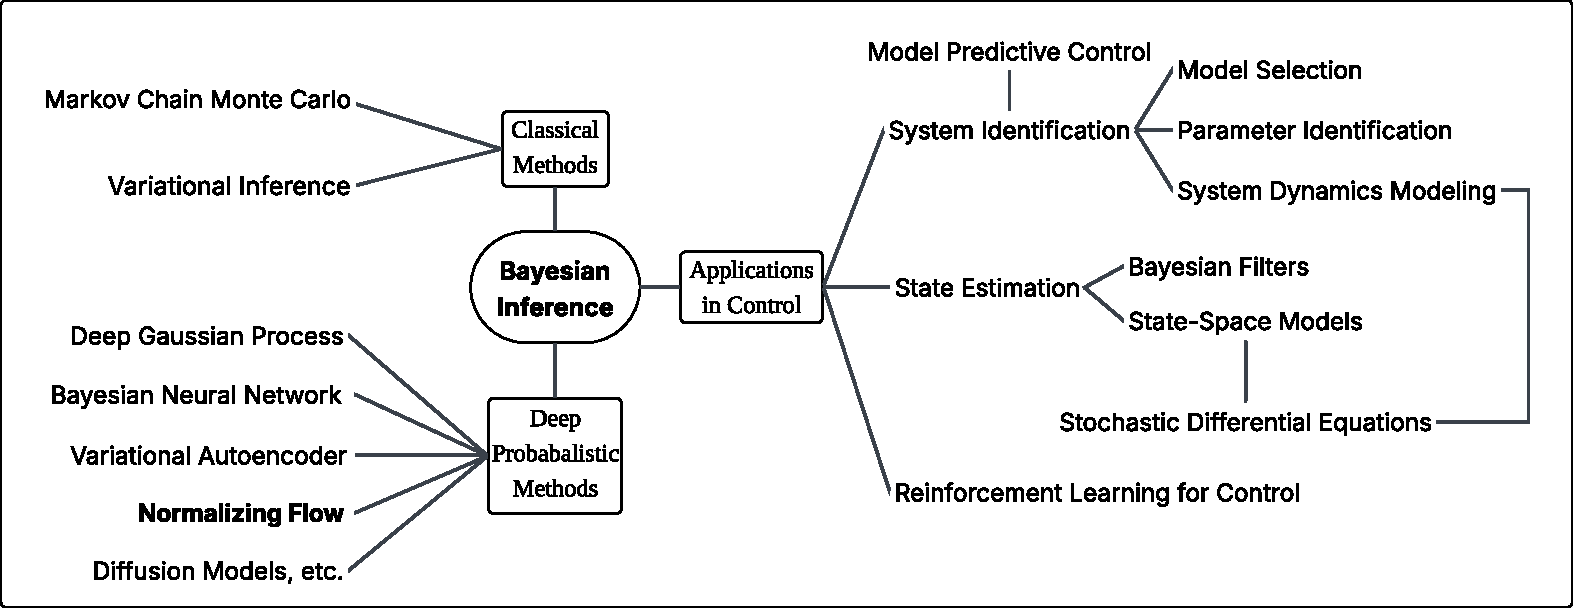
\includegraphics[width=\textwidth]{figures/Mindmap.pdf}
    \caption[Knowledge Map]{Knowledge Map of Foundational Theories}
    \label{fig:knowledgemap}
\end{figure}
This section introduces the necessary foundational concepts and methodologies for understanding the rest of this work. Before the main contents, we explain the unified notations applied in this whole work. We first review classical Bayesian inference methods. Then we introduce deep probabilistic methods, including \acf{DGP}, \acf{BNN}, and \acf{VAE}. Next, we present the core methods of this work, \acfp{NF}, a powerful class of generative models for flexible density estimation. Finally, we bridge Bayesian inference to control methods, covering system identification, state estimation, and model predictive control. The overview for this chapter is shown in Figure~\ref{fig:knowledgemap}.

\subsection{Notations}

To maintain clarity throughout this document, we adopt the following notation:

\begin{table}[htbp!]
\centering
\renewcommand{\arraystretch}{1.5}
\begin{tabularx}{0.9\textwidth}{>{\bfseries}l X}
\toprule
Category & Description \\
\midrule
Basic Symbols &
Scalars: $x$; Vectors: $\boldsymbol{x}$; Matrices: $\boldsymbol{X}$; Sets: $\mathcal{D}$ \\
\midrule
Random Variables &
Multidimensional random variables: $\boldsymbol{x} = [x_1,\dots,x_N]^T$; Sample index: $\boldsymbol{x}^{(i)}$; Stochastic processes: $\it{X}(t)$ \\
\midrule
Time Series &
Time series of length $T$: $\boldsymbol{x}_{(1:T)}$; Time-dependent variables: $\boldsymbol{x}(t)$ or $x(t)$; Dimension index: $\boldsymbol{x}_i$ \\
\midrule
Variable Modifications &
Estimated: $\hat{\boldsymbol{x}}$; Transformed: $\tilde{\boldsymbol{x}}$; Time derivative: $\dot{\boldsymbol{x}}$ \\
\midrule
Probability and Statistics &
PDF: $p(\cdot)$; Joint PDF: $p(\cdot, \cdot)$; Conditional PDF: $p(\cdot \mid \cdot)$; Expectation: $\mathbb{E}_{p(x)}[f(x)]$; Covariance: $\text{Cov}[\boldsymbol{x}, \boldsymbol{y}]$; Variance: $\text{Var}[\boldsymbol{x}]$ \\
\midrule
Matrix Operations &
Identity: $\boldsymbol{I}$; Jacobian: $\boldsymbol{J}$; Determinant: $\det|\boldsymbol{J}|$; Trace: $\text{Tr}(\boldsymbol{X})$; Transpose: $\boldsymbol{X}^\top$ \\
\bottomrule
\end{tabularx}
\caption{Notation Summary}
\label{tab:notation-summary}
\end{table}

\subsection{Bayesian Inference}
Bayesian inference gets its name from using Bayes' rule to perform statistical inference of probability distributions.
This chapter refers to \textit{Bayesian Data Analysis} \citep{gelman2013bayesian}, \textit{Handbook of MCMC} \citep{Allen_2007}, and \textit{Variational Inference} \citep{Blei_2017}.

\subsubsection{Bayes' Rule}
Bayes' rule is derived from the chain rule of conditional probability. For target variables $\boldsymbol{\theta}$ and the corresponding observed data $\mathcal{D}$, the chain rule states that:
\begin{equation}
    p(\boldsymbol{\theta}, \mathcal{D}) = p(\boldsymbol{\theta}|\mathcal{D})p(\mathcal{D}) = p(\mathcal{D}|\boldsymbol{\theta})p(\boldsymbol{\theta}).
\end{equation}
Rearranging the terms gives Bayes' rule or Bayes' theorem:
\begin{equation}
\label{eq:bayes}
    p(\boldsymbol{\theta}|\mathcal{D})= \frac{p(\mathcal{D}|\boldsymbol{\theta})p(\boldsymbol{\theta})}{p(\mathcal{D})}.
\end{equation}
In Bayes' theorem, $p(\boldsymbol{\theta})$ is the initial distribution of the variables before any data samples are considered, which is called the prior distribution. $p(\boldsymbol{\theta}|\mathcal{D})$ is the posterior distribution of the target parameter after being updated by the observed data. $p(\mathcal{D}|\boldsymbol{\theta})$ is the likelihood of expected data given the setting of parameters $\boldsymbol{\theta}$. $p(\mathcal{D})$ is called the marginal likelihood or evidence of expected data across all possible parameter settings:
\begin{subequations}
    \begin{align}
    p(\mathcal{D}) &= \Sigma_{\boldsymbol{\theta}'}p(D|\boldsymbol{\theta}')p(\boldsymbol{\theta}')\Delta \boldsymbol{\theta}',\\
    p(\mathcal{D}) &= \int p(D|\boldsymbol{\theta}')p(\boldsymbol{\theta}')d\boldsymbol{\theta}'.
    \end{align}
\end{subequations}
In practice, it is often treated as a normalizing constant and ignored. The unnormalized posterior is then given by:
\begin{equation}
    p_u(\boldsymbol{\theta}|\mathcal{D}) \propto p(\mathcal{D}|\boldsymbol{\theta})p(\boldsymbol{\theta}).            
\end{equation}

Normally, the posterior distribution does not have a closed-form expression. Instead, we approximate it using numerical methods. Computational algorithms that rely on repeated random sampling to obtain numerical results refers to "Monte Carlo" methods. Monte Carlo methods provide ways to approximate the posterior distribution by expectations:
\begin{equation}
    E=\mathbb{E}_{p(\boldsymbol{\theta}|\mathcal{D})}[f(\boldsymbol{\theta})] = \int f(\boldsymbol{\theta}) p(\boldsymbol{\theta}|\mathcal{D}) d\boldsymbol{\theta},
\end{equation}
where $f(\boldsymbol{\theta})$ is any function of interest, for example, $f(\boldsymbol{\theta})=\boldsymbol{\theta}$. As the simplest way, we can approximate it using standard numerical techniques such as a Riemann sum over a discrete grid of points:
\begin{equation}
    E \approx \Sigma_{\boldsymbol{\theta}'} f(\boldsymbol{\theta}') \Delta \boldsymbol{\theta}'.
\end{equation}
However, this approach is only feasible for low-dimensional $\boldsymbol{\theta}$ due to the curse of dimensionality. Besides, for complex distributions, the discretization is highly inefficient. Therefore, for high-dimensional parameters and complex distributions, we often resort to sampling-based or optimization-based methods to approximate the posterior distribution, which will be discussed in the following sections.

\subsubsection{Markov Chain Monte Carlo}
The "Markov Chain" aspect indicates that these algorithms generate a sequence of samples where each sample depends only on the previous one. In contrast to the basic Monte Carlo methods, \acf{MCMC} methods produce auto-correlated samples, so that each new sample adds less new information than an independent draw would. Different sequences updating algorithms lead to different \ac{MCMC} methods. The goal of \ac{MCMC} is to construct a Markov chain that has the desired posterior distribution as its equilibrium distribution. After running the chain for a sufficient number of iterations, the samples generated from the chain can be treated as samples from the target posterior distribution.

\paragraph{\acf{MH} algorithm}
The \ac{MH} algorithm, which is named after Metropolis \citeyearpar{Metropolis} and Hastings \citeyearpar{Hastings}, is a widely used \ac{MCMC} method. The steps of the \ac{MH} algorithm are as follows:
\begin{enumerate}
    \item Initialize the chain with a starting point $\boldsymbol{\theta}_{(0)}$, choose a proposal distribution $q(\boldsymbol{\theta}'|\boldsymbol{\theta})$. 
    \item For each iteration $i$:
    \begin{enumerate}
        \item Propose a new state $\boldsymbol{\theta}'_{(i)}$ from the proposal distribution $q(\boldsymbol{\theta}'_{(i)}|\boldsymbol{\theta}_{(i-1)})$.             
        \item Calculate the transition probability, also known as the acceptance ratio: 
        \begin{equation}
        \label{eq:mh_transition}
        T(\boldsymbol{\theta}'_{(i)}|\boldsymbol{\theta}_{(i-1)})=\min\{1, \frac{p(\boldsymbol{\theta}'_{(i)}|\mathcal{D})q(\boldsymbol{\theta}_{(i-1)}|\boldsymbol{\theta}'_{(i)})}{p(\boldsymbol{\theta}_{(i-1)}|\mathcal{D})q(\boldsymbol{\theta}'_{(i)}|\boldsymbol{\theta}_{(i-1)})}\}.
        \end{equation}
        \item Generate a uniform random number $u \sim U(0,1)$. Update $\boldsymbol{\theta}_{(i)}$ by "accept or reject":
        \begin{equation}
            \label{eq:mh_update}
        \boldsymbol{\theta}_{(i)} = \begin{cases} \boldsymbol{\theta}'_{(i)}, & \text{if } u < T(\boldsymbol{\theta}'_{(i)}|\boldsymbol{\theta}_{(i-1)}) \\ \boldsymbol{\theta}_{(i-1)}, & \text{otherwise} \end{cases}.
        \end{equation} 
    \end{enumerate}
    \item Repeat step 2 for numerous iterations to obtain a sequence of samples $\{\boldsymbol{\theta}_{(1)}, \ldots, \boldsymbol{\theta}_{(N)}\}$.
\end{enumerate}
From the sequence of samples, we can construct a Monte Carlo estimator:
\begin{equation}
    p(\boldsymbol{\theta}| \mathcal{D}) \approx \frac{1}{N} \Sigma_{i=1}^{N} \delta_{\boldsymbol{\theta}_{(n)}}(\boldsymbol{\theta}).
\end{equation}
Although this procedure allows flexible approximation of complex posterior distribution, it suffers from slow convergence rate due to its random exploration nature. Thus, gradient-based \ac{MCMC} methods are proposed to incorporate the structure of the target density, leading to faster sampling.

\paragraph{\acf{MALA}}\label{sec:MALA}
The \ac{MALA} \citep{besag2004markov} combines the \ac{MH} algorithm with Langevin diffusion, whose stationary distribution is the target density. In general, for a stochastic process $\Theta(t)$, the Langevin diffusion is described by the following \ac{SDE}:
\begin{equation}
d\Theta(t)=\nabla \log p(\Theta(t))dt + \sqrt{2} dW(t),
\end{equation}
where $W(t)$ denotes a standard Wiener process \citep{gabbiani2010mathematics}. The Wiener process is a continuous-time stochastic process with independent, normally distributed increments, which can be interpreted as Brownian motion. It has the following properties:
\begin{enumerate}
    \item [(1)] $W(0)=\boldsymbol{0}$;
    \item [(2)] for $t > s \geq 0 $, $W(t)-W(s)\sim\sqrt{t-s}\;\mathcal{N}(\boldsymbol{0}, \boldsymbol{I})$;
    \item [(3)] for $t_1>s_1\geq 0$, and $t_2>s_2\geq 0$, $W(t_1)-W(s_1)$ and $W(t_2)-W(s_2)$ are independent. 
\end{enumerate}                 
The \ac{MALA} algorithm uses the first order Euler-Maruyama discretization of the \ac{SDE}, resulting in the following proposal distribution:
\begin{equation}
    \label{eq:langevin}
    \Theta(t) = \Theta(i-1) + \tau \nabla \log p(\Theta(i-1)) + \sqrt{2\tau}\; \mathcal{N}(\boldsymbol{0}, \boldsymbol{I}),
\end{equation}
where $\tau$ is a step size parameter.
Because of the discretization, convergence to the target density is no longer guaranteed. Therefore, the \ac{MH} algorithm is applied to correct the bias introduced by the discretization. 
For each iteration $i$, the \ac{MALA} algorithm updates the state as follows:
\begin{enumerate}
    \item[(a)] Compute the gradient of the log-posterior at the current state: $\nabla \log p(\boldsymbol{\theta}_{(i-1)}|\mathcal{D})$.
    \item[(b)] Propose a new state $\boldsymbol{\theta}'_{(i)}$ using the Langevin dynamics (\ref{eq:langevin}).
    \item[(c)] Calculate the transition probability according to Equation \ref{eq:mh_transition}. Specifically, the proposal distribution is derived from the Langevin dynamics:
    \begin{equation}
        q(\boldsymbol{\theta}'_{(i)}|\boldsymbol{\theta}_{(i-1)})\propto \exp(-\frac{1}{4\tau}\left\|\boldsymbol{\theta}'_{(i)}-\boldsymbol{\theta}_{(i-1)}-\tau\nabla\log p(\boldsymbol{\theta}_{(i-1)}|\mathcal{D})\right\|^2_2).
    \end{equation}
    \item[(d)] (same as MCMC) Generate a uniform random number $u \sim U(0,1)$. Update $\boldsymbol{\theta}_{(i)}$ by "accept or reject" according to Equation \ref{eq:mh_update}. 
\end{enumerate}

Compared to the \ac{MH}, \ac{MALA} converges faster and scales better in higher dimensions, at the cost of requiring gradients and tuning. As a more advanced \ac{MCMC} method, \acf{HMC} \citep{duane1987hybrid} further improves sampling efficiency by simulating the whole sampling trajectory as Hamiltonian dynamics. 

\subsubsection{Variational Inference}
Different from \ac{MCMC}, \acf{VI} \citep{Jordan1998, Wainwright2008} is an optimization-based method that approximates the target posterior distribution $p(\boldsymbol{\theta}|\mathcal{D})$ with a simpler, parameterized distribution $q_{\boldsymbol{\phi}}(\boldsymbol{\theta})$, where $\boldsymbol{\phi}$ are the variational factors. The goal of \ac{VI} is to find the optimal variational factors $\boldsymbol{\phi}^*$ that minimize the distance between the approximate distribution and the true posterior. The distance is normally measured by the \ac{KL}-divergence \citep{kl1951}, which is defined as:
\begin{equation}
    D_{\text{KL}}(q(z)||p(z)) = \mathbb{E}_{q(z)}[\log \frac{q(z)}{p(z)}] = \int q(z)\log \frac{q(z)}{p(z)}dz.
\end{equation}
Thus, the optimization problem of \ac{VI} can be formulated as:
\begin{equation}
    \boldsymbol{\phi}^* = \arg\min_{\boldsymbol{\phi}} D_{\text{KL}} (q_{\boldsymbol{\phi}}(\boldsymbol{\theta}) || p(\boldsymbol{\theta}|\mathcal{D})).
\end{equation}
Substituting Bayes' rule (\ref{eq:bayes}) into \ac{KL}-divergence, we have:
\begin{equation}
    D_{\text{KL}} (q_{\boldsymbol{\phi}}(\boldsymbol{\theta}) || p(\boldsymbol{\theta}|\mathcal{D})) = D_{\text{KL}} (q_{\boldsymbol{\phi}}(\boldsymbol{\theta}) || \frac{p(\mathcal{D}|\boldsymbol{\theta})p(\boldsymbol{\theta})}{p(\mathcal{D})}).
\end{equation}
The marginal likelihood $p(\mathcal{D})$ is usually intractable, as it involves integrating over all possible parameter settings. Therefore, the divergence cannot be computed directly.

Expanding the above equation with the definition of \ac{KL}-divergence, we have:
\begin{multline}
    D_{\text{KL}}(q_{\boldsymbol{\phi}}(\boldsymbol{\theta}) || p(\boldsymbol{\theta}|\mathcal{D})) = \mathbb{E}_{q_{\boldsymbol{\phi}}(\boldsymbol{\theta})}[\log q_{\boldsymbol{\phi}}(\boldsymbol{\theta}) - \log p(\mathcal{D}|\boldsymbol{\theta}) - \log p(\boldsymbol{\theta}) + \log p(\mathcal{D})]\\
    = \mathbb{E}_{q_{\boldsymbol{\phi}}(\boldsymbol{\theta})}\log q_{\boldsymbol{\phi}}(\boldsymbol{\theta})-\mathbb{E}_{q_{\boldsymbol{\phi}}(\boldsymbol{\theta})}\log p(\mathcal{D}|\boldsymbol{\theta})-\mathbb{E}_{q_{\boldsymbol{\phi}}(\boldsymbol{\theta})}\log p(\boldsymbol{\theta}) + \mathbb{E}_{q_{\boldsymbol{\phi}}(\boldsymbol{\theta})}\log p(\mathcal{D}).
\end{multline}
Since $p(\mathcal{D})$ is independent of the variational factors $\boldsymbol{\phi}$, the last term is reduced to $\log p(\mathcal{D})$.
Combining the terms $p(\mathcal{D}|\boldsymbol{\theta})p(\boldsymbol{\theta})=p(\boldsymbol{\theta}, \mathcal{D})$ gives
\begin{equation}
    \label{eq:vi_kl1}
    D_{\text{KL}}(q_{\boldsymbol{\phi}}(\boldsymbol{\theta}) || p(\boldsymbol{\theta}|\mathcal{D})) = \mathbb{E}_{q_{\boldsymbol{\phi}}(\boldsymbol{\theta})}\log q_{\boldsymbol{\phi}}(\boldsymbol{\theta})-\mathbb{E}_{q_{\boldsymbol{\phi}}(\boldsymbol{\theta})}\log p(\boldsymbol{\theta}, \mathcal{D}) + \log p(\mathcal{D})
\end{equation}
Or combining the terms $q_{\boldsymbol{\phi}}(\boldsymbol{\theta})$ and $p(\boldsymbol{\theta})$ via \ac{KL}-divergence  gives:
\begin{equation}
    \label{eq:vi_kl2}
    D_{\text{KL}}(q_{\boldsymbol{\phi}}(\boldsymbol{\theta}) || p(\boldsymbol{\theta}|\mathcal{D}))=D_{\text{KL}}(q_{\boldsymbol{\phi}}(\boldsymbol{\theta})||p(\boldsymbol{\theta})) - \mathbb{E}_{q_{\boldsymbol{\phi}}(\boldsymbol{\theta})}\log p(\mathcal{D}|\boldsymbol{\theta}) + \log p(\mathcal{D})
\end{equation}
Rearranging the terms in Equation \ref{eq:vi_kl1} gives:
\begin{equation}
    \log p(\mathcal{D}) = D_{\text{KL}}(q_{\boldsymbol{\phi}}(\boldsymbol{\theta}) || p(\boldsymbol{\theta}|\mathcal{D}))+\mathbb{E}_{q_{\boldsymbol{\phi}}(\boldsymbol{\theta})}\log p(\boldsymbol{\theta}, \mathcal{D})-\mathbb{E}_{q_{\boldsymbol{\phi}}(\boldsymbol{\theta})}\log q_{\boldsymbol{\phi}}(\boldsymbol{\theta}).
\end{equation} 
Since the \ac{KL}-divergence is always non-negative, we have:
\begin{equation}
    \label{eq:elbo1}
    \log p(\mathcal{D}) \geq \mathbb{E}_{q_{\boldsymbol{\phi}}(\boldsymbol{\theta})}\log p(\boldsymbol{\theta}, \mathcal{D})-\mathbb{E}_{q_{\boldsymbol{\phi}}(\boldsymbol{\theta})}\log q_{\boldsymbol{\phi}}(\boldsymbol{\theta}).
\end{equation}
Because of this inequality, the right hind side is called the \acf{ELBO}, also known as the variational lower bound. Another way to formulate the \ac{ELBO} using Equation \ref{eq:vi_kl2} is:
\begin{equation}
    \label{eq:elbo2}
    \text{ELBO} = \mathbb{E}_{q_{\boldsymbol{\phi}}(\boldsymbol{\theta})}\log p(\mathcal{D}|\boldsymbol{\theta}) - D_{\text{KL}}(q_{\boldsymbol{\phi}}(\boldsymbol{\theta})||p(\boldsymbol{\theta})). 
\end{equation}
Then, minimizing the \ac{KL}-divergence is equivalent to maximizing the \ac{ELBO} (\ref{eq:elbo1}), leading to the equivalent optimization problem:
\begin{equation}
    \label{eq:vi_opt}
    \boldsymbol{\phi}^* = \arg\max_{\boldsymbol{\phi}} \text{ELBO} = \arg\min_{\boldsymbol{\phi}}[\mathbb{E}_{q_{\boldsymbol{\phi}}(\boldsymbol{\theta})}\log q_{\boldsymbol{\phi}}(\boldsymbol{\theta})-\mathbb{E}_{q_{\boldsymbol{\phi}}(\boldsymbol{\theta})}\log p(\boldsymbol{\theta}, \mathcal{D})].
\end{equation}

To complete the optimization, we need to choose a suitable family of variational distributions $q_{\boldsymbol{\phi}}(\boldsymbol{\theta})$. A common choice is the mean-field family \citep{bishop2006}, which assumes that the variables $\boldsymbol{\theta}$ are mutually independent and each governed by a distinct factor under $q$:
\begin{equation}
    q_{\boldsymbol{\phi}}(\boldsymbol{\theta}) = \Pi_{i} q_{\phi_i}(\theta_i),
\end{equation}
where each factor $\phi_i$ governs a variable $\theta_i$. Then, the \ac{ELBO} (\ref{eq:elbo1}) is iteratively optimized by updating each factor while holding the others fixed. The solution of the optimal distribution $q_{\phi_i}(\theta_i)$ is proportional to the exponential expected log of the complete condition:
\begin{equation}
    \log q_{\phi_i}^*(\theta_i) \propto \mathbb{E}_{\Pi_{j\neq i}q_{\phi_i}(\theta_i)}[\log p(\theta_i|\boldsymbol{\theta}_{j\neq i}, \mathcal{D})],
\end{equation}
where the expectation is taken with respect to the distributions of all other groups $j \neq i$. This algorithm is called \ac{CAVI} \citep{bishop2006}. 

The assumption of the mean-field \ac{VI} simplifies the optimization problem, and thus makes it scalable for large dimensional variables and also enables parallelizable computation. However, it may also limit the expressiveness of the variational distribution, especially when the posterior correlations are crucial, leading to suboptimal approximations of the true posterior. Summarizing, \ac{VI} is generally faster than \ac{MCMC} and scales better to large datasets, but it may provide less accurate approximations of the posterior distribution \citep{Blei_2017}. 

\subsection{Deep Probabilistic Methods}
\label{sec:introduction:background:deep_probabilistic_methods}
The classical methods, \ac{MCMC} and \ac{VI}, although provide general solution for Bayesian inference, they are limited by their "approximation-per-point" behavior. Deep probabilistic methods, on the contrary, enable amortized Bayesian inference and unlock both high expressiveness and scalability to large datasets. In the following section, we briefly review three prominent deep probabilistic methods: the Deep Gaussian Process, the Bayesian Neural Network, and the Variational Autoencoder. The former two methods are direct extensions of classical Bayesian inference with deep architectures, while the last one is a fundamental deep generative model that leverages variational inference.

\subsubsection{Deep Gaussian Process}
A Gaussian process can be interpreted as an infinite-dimensional Gaussian distribution, where at each time point the random variables follow normal distributions. For an $N$-dimensional random variable $\boldsymbol{x}=[x_1,\dots,x_N]^T$, a Gaussian process $\it{X}(t)$ is fully specified by its mean function $\mu(\cdot)$ and covariance function $k(\cdot, \cdot)$:
\begin{equation}
     \begin{bmatrix} \it{X}_1(t) \\ \cdots \\\it{X}_N(t) \end{bmatrix}\sim\mathcal{N}( \begin{bmatrix} \mu(x_1) \\ \cdots \\\mu(x_N) \end{bmatrix},  \begin{bmatrix} k(x_1,x_1),\dots,k(x_1, x_N) \\ \cdots \\k(x_N,x_1), \dots,k(x_N, x_N) \end{bmatrix})
\end{equation}
Using a Gaussian process to infer variables from observed data based on prior distributions leads to \ac{GPR} \citep{Rasmussen_Williams_2008}. For a regression task with training data $\boldsymbol{x}$ and the ground truth $\boldsymbol{y}$, the \ac{GPR} model is employed by a latent function $f(\cdot)$:
\begin{equation}
    \label{eq:simgp}
    y_i = f(x_i) + \epsilon_i,\quad i=1,\dots,N,
\end{equation}
where $\epsilon_i \sim \mathcal{N}(0, \sigma_\epsilon^2)$ are \ac{i.i.d.} noises for all dimensions. We denote the collection of latent functions as $\boldsymbol{f}=[f(x_1), \dots, f(x_N)]^T$. So, the likelihood of $\boldsymbol{y}$ is given by:
\begin{equation}
    p(\boldsymbol{y}|\boldsymbol{f}) = \prod_{i=1}^{N}p(y_i|f(x_i)) = \prod_{i=1}^{N}\mathcal{N}(y_i|f(x_i), \sigma_\epsilon^2).    
\end{equation}                                                                                                                          
The prior distribution over functions $f(\cdot)$ is assumed to a zero-mean Gaussian process. We denote it as:
\begin{equation}
    f(\cdot) \sim \mathcal{GP}(0, k(\cdot, \cdot)).
\end{equation}
The kernel function $k(\cdot, \cdot)$ is usually chosen to be the \ac{SE} kernel function, or as known as the \ac{RBF}, defined as:
\begin{equation}
    k(x_i, x_j) = \sigma_{SE}^2\exp(-\frac{1}{2\ell^2}\left\|x_i - x_j\right\|^2),
\end{equation}
where $\sigma_{SE}$ and $\ell$ are vertical and horizontal scale parameters, which control the vertical span and smoothness of the function, respectively. Then, the posterior distribution of $\boldsymbol{y}$ can be computed analytically using the marginal likelihood over $\boldsymbol{y}$:
\begin{equation}
    p(\boldsymbol{y}|\boldsymbol{x}) = \int \prod_{i=1}^{N}p(y_i|f(x_i))p(f(x_i)|x_i)d\boldsymbol{f}=\mathcal{N}(\boldsymbol{y}|\boldsymbol{0},\boldsymbol{K}+\sigma_\epsilon^2\mathbb{I}), \quad \boldsymbol{K}=k(\boldsymbol{x}, \boldsymbol{x}).
\end{equation}
The hyperparameters $\boldsymbol{\phi}=\{\sigma_{SE}, \ell, \sigma_\epsilon\}$ can be optimized by maximizing the log marginal likelihood $\log p(\boldsymbol{y}|\boldsymbol{x}, \boldsymbol{\phi})$.

The \ac{GPR} is widely used for regression tasks owing to its non-parametric nature and its capacity to quantify uncertainty. However, its computational complexity scales cubically with the number of training points, i.e., $\mathcal{O}(N^3)$ for an $N$-dimensional input. Additionally, calculating the Gaussian processes requires the entire storage of training datasets, incurring a memory cost of $\mathcal{O}(M^2)$, which grows quadratically with the dataset size $M$. These limitations hinder its scalability to high-dimensional inputs and large datasets. In addition, the expressiveness of \ac{GPR} is constrained by the choice of kernel function and its incapacity to perform hierarchical feature extraction.

To improve expressiveness, \ac{DGP} \citep{damianou2013dgp} is proposed as multilayer hierarchical generalizations of Gaussian processes. The input $\boldsymbol{x}$ is passed through multiple layers of Gaussian processes to obtain the output $\boldsymbol{y}$. For an $L$-layer \ac{DGP}, the model extends the Gaussian process (\ref{eq:simgp}) by:
\begin{multline}
    y_i = f_{L}(f_{L-1}(\dots f_{1}(x_i)+\epsilon_{i,1}\dots)) + \epsilon_{L}, \quad f_{l}(\cdot) \sim \mathcal{GP}(0, k_l(\cdot, \cdot)), \\ l=1,\dots,L,\; i=1,\dots,n.
\end{multline}  
The deep architecture enables Gaussian processes to learn more complex data patterns and hierarchical representations. It can be seen as a deep neural network with infinitely wide layers \citep{Neal1996}, where each layer applies a Gaussian process, instead of nonlinear matrix transformation. However, due to the computational cost and storage consumption the \ac{DGP} is still cumbersome to apply in practice. 

\subsubsection{Bayesian Neural Network}
Another approach of deep probabilistic methods involves integrating Bayesian inference with deep neural networks. A \acf{BNN} \citep{Neal1996, MacKay1992} places prior distributions over the network’s weights and biases, allowing uncertainty to be modeled directly within the architecture. 

The goal of training a \ac{BNN} is to infer the posterior distribution over the parameters $\boldsymbol{\theta}=[\boldsymbol{w}, \boldsymbol{b}]$ given the training data $\mathcal{D}$, i.e., $p(\boldsymbol{\theta}|\mathcal{D})$. \ac{VI} is commonly employed to approximate the posterior by optimizing the \ac{ELBO} (\ref{eq:elbo2}). 
To facilitate gradient-based optimization via backpropagation---similar to standard neural networks---the reparameterization trick \citep{kingma2013auto} is used. This technique expresses random variables as deterministic variables of noise, enabling efficient and differentiable sampling during training. For example, for a Gaussian variational distribution $q_{\boldsymbol{\phi}}(\boldsymbol{\theta})=\mathcal{N}(\boldsymbol{\theta}|\boldsymbol{\mu}, \text{diag}(\boldsymbol{\sigma}^2))$, we can reparameterize $\boldsymbol{\theta}$ as:  
\begin{equation}
    \boldsymbol{\theta} = \boldsymbol{\mu} + \boldsymbol{\sigma} \odot \boldsymbol{\epsilon}, \quad \boldsymbol{\epsilon}\sim\mathcal{N}(\boldsymbol{0}, \boldsymbol{I}),
\end{equation}  
where $\odot$ represents the Hadamard product, i.e., the element-wise product, and the variational parameters here are $\boldsymbol{\phi}=[\boldsymbol{\mu}, \boldsymbol{\sigma}]$. 
To train a \ac{BNN} on large datasets, \ac{SGD} \citep{bottou1999sgd} is typically employed to optimize the \ac{ELBO}. Unlike standard gradient descent, \ac{SGD} estimates the gradient at each iteration using a randomly selected subset of the data. Then, the variational objective of a \ac{BNN} using the \ac{ELBO} (\ref{eq:elbo2}) becomes:
\begin{equation}
    \mathcal{L}(\boldsymbol{\theta}, \boldsymbol{\phi}) = \frac{1}{M}\sum_{i=1}^{M} [D_{\text{KL}}(q_{\boldsymbol{\phi}}(\boldsymbol{\theta})||p(\boldsymbol{\theta}))-\mathbb{E}_{q_{\boldsymbol{\phi}}(\boldsymbol{\theta})}\log p(\mathcal{D}_i|\boldsymbol{\theta})],
\end{equation}
where each mini-batch $\mathcal{D}_i\subset\mathcal{D}$ is drawn from the equally sized subsets of the training data $\mathcal{D}=\{\mathcal{D}_1,\dots,\mathcal{D}_M\}$. During each optimization step, the auxiliary noise $\boldsymbol{\epsilon}$ is sampled multiple times from $\mathcal{N}(\boldsymbol{0}, \boldsymbol{I})$ to perform Monte Carlo estimation of the expectation terms in the loss function $\mathcal{L}(\boldsymbol{\theta}, \boldsymbol{\phi})$. The gradient $\nabla_{\boldsymbol{\phi}}\mathcal{L}(\boldsymbol{\theta}, \boldsymbol{\phi})$ is then computed via backpropagation and averaged across all samples. Finally, the variational parameter $\boldsymbol{\phi}$ is updated by 
\begin{equation}
    \boldsymbol{\phi}\leftarrow\boldsymbol{\phi}-\alpha\nabla_{\boldsymbol{\phi}}\mathcal{L}(\boldsymbol{\theta}, \boldsymbol{\phi}),
\end{equation}
where $\alpha$ is the learning rate. This procedure is called \ac{BbB} \citep{blundell2015bbb}.

In comparison to \ac{DGP}, the \ac{BNN} demonstrates better scalability to large datasets and improved representational capacity. Moreover, the \ac{BbB} method facilitates the compatibility of \ac{BNN} with deep learning techniques and thus enables flexible implementation in different neural network architectures, such as \ac{CNN} \citep{shridhar2019bcnn}, \ac{RNN} \citep{fortunato2019brnn}, and Transformer \citep{müller2024transbi}. Nevertheless, several works raise concerns with BNNs including wrong uncertainty estimation in between separated regions of observations \citep{foong2019inbetween, foong2020bnn}, poor generalization ability under domain shift \citep{izmailov2021bnnp}, and sensitive modeling ability to the choice of prior distributions \citep{silvestro2020prior}. These limitations motivate the applications of more powerful generative models, such as variational autoencoders and \acp{NF}, which are discussed in the following sections.

\subsubsection{Variational Autoencoder}
In classical \ac{VI} methods, the parameters of interest $\boldsymbol{\theta}$ are random variables, and the approximate posterior distribution over the parameters is parameterized by variational parameters $\boldsymbol{\phi}$. In contrast, a \acf{VAE} is constructed with deterministic neural networks and introduces variability by latent variables. For a dataset $\mathcal{D}=\{\boldsymbol{x}^{(i)}\}_{i=1}^{N}$, the samples are assumed to be \ac{i.i.d.} and drawn from an unchanging underlying distribution $p_{\boldsymbol{\theta}}(\boldsymbol{x})$. A \ac{VAE} extracts information from input data $\boldsymbol{x}$ to latent variables $\boldsymbol{z}$ by a parameterized inference model $q_{\boldsymbol{\phi}}(\boldsymbol{z}|\boldsymbol{x})$, which is also called an encoder or recognition model. Then, the \ac{VAE} generates data $\boldsymbol{x}$ from the latent variables $\boldsymbol{z}$ by another parameterized model $p_{\boldsymbol{\theta}}(\boldsymbol{x}|\boldsymbol{z})$, which is also called a decoder. The decoder is often mentioned as a "generative" model. However, according to the formal definition \citep{Kingma_2019}, a generative model learns a joint distribution $p_{\boldsymbol{\theta}}(\boldsymbol{z}, \boldsymbol{x})=p_{\boldsymbol{\theta}}(\boldsymbol{z})p_{\boldsymbol{\theta}}(\boldsymbol{x}|\boldsymbol{z})$, including sampling $\boldsymbol{z}\sim p_{\boldsymbol{\theta}}(\boldsymbol{z})$ and sampling $\boldsymbol{x}\sim p_{\boldsymbol{\theta}}(\boldsymbol{x}|\boldsymbol{z})$. 

The latent variables connect the inference model and the generative model. From the encoder side, the inference model $q_{\boldsymbol{\phi}}(\boldsymbol{z}|\boldsymbol{x})$ approximates the true posterior distribution $p_{\boldsymbol{\theta}}(\boldsymbol{z}|\boldsymbol{x})$ of the generative model, which is intractable. From the decoder side, the distribution of latent variables is a prior distribution, which is usually chosen to be a standard normal distribution, i.e., $p(\boldsymbol{z})=\mathcal{N}(\boldsymbol{z}|\boldsymbol{0}, \boldsymbol{I})$. The whole architecture is illustrated in Figure~\ref{fig:vae}.
\begin{figure}[htp!]
    \centering
    \includegraphics[width=0.8\textwidth]{figures/VAE.pdf} 
    \caption[Variational Autoencoder Architecture]{The architecture of a Variational Autoencoder. The encoder (with neural network parameters $\boldsymbol{\phi}$) maps the input data $\boldsymbol{x}$ to latent variables $\boldsymbol{z}$, and the decoder (with neural network parameters $\boldsymbol{\theta}$) reconstructs the input data from the latent variables.}
    \label{fig:vae}
\end{figure}

Same reparameterization trick as in the \ac{BNN} is used to enable gradient-based optimization. The latent variables $\boldsymbol{z}$ becomes:
\begin{equation}
    \boldsymbol{z} = \boldsymbol{\mu}_{\boldsymbol{\phi}}(\boldsymbol{x}) + \boldsymbol{\sigma}_{\boldsymbol{\phi}}(\boldsymbol{x}) \odot \boldsymbol{\epsilon}, \quad \boldsymbol{\epsilon}\sim\mathcal{N}(\boldsymbol{0}, \boldsymbol{I}),
\end{equation}
where $\boldsymbol{\mu}_{\boldsymbol{\phi}}(\boldsymbol{x})$ and $\boldsymbol{\sigma}_{\boldsymbol{\phi}}(\boldsymbol{x})$ are also neural networks. 
Different from the mini-batch optimization in the \ac{BNN}, we use one single encoder neural network to perform posterior inference over all samples in the dataset. This strategy of sharing variational parameters across datapoints is called amortized variational inference \citep{gershman2014amortized, margossian2024amortized}, which improves the optimization efficiency. 

The objective of the inference model is to minimize the \ac{KL}-divergence between the inferred and true posterior $D_{\text{KL}}(q_{\boldsymbol{\phi}}(\boldsymbol{z}|\boldsymbol{x})||p_{\boldsymbol{\theta}}(\boldsymbol{z}|\boldsymbol{x}))$. Recall the \ac{ELBO} in \ac{VI} (\ref{eq:elbo1}, \ref{eq:elbo2}), the \ac{ELBO} of a \ac{VAE} is given by:
\begin{equation}
    \log p_{\boldsymbol{\theta}}(\boldsymbol{x}) \geq \mathbb{E}_{q_{\boldsymbol{\phi}}(\boldsymbol{z}|\boldsymbol{x})}\log p_{\boldsymbol{\theta}}(\boldsymbol{x}|\boldsymbol{z}) - D_{\text{KL}}(q_{\boldsymbol{\phi}}(\boldsymbol{z}|\boldsymbol{x})||p_{\boldsymbol{\theta}}(\boldsymbol{z})).
\end{equation}
Maximizing the \ac{ELBO} optimizes concurrently both the inference model and the generative model. The marginal likelihood $p_{\boldsymbol{\theta}}(\boldsymbol{\theta})$ is maximized, meaning the generated data maximally resembles the input data. Meanwhile, the distance between the approximated and the true posterior is minimized. 
Changing the prior distribution in the \ac{ELBO}, $p_{\boldsymbol{\theta}}(\boldsymbol{z}):=p(\boldsymbol{z})$, the overall loss function of a \ac{VAE} is given by:
\begin{equation}
    \mathcal{L}(\boldsymbol{\theta}, \boldsymbol{\phi}) = -\mathbb{E}_{q_{\boldsymbol{\phi}}(\boldsymbol{z}|\boldsymbol{x})}\log p_{\boldsymbol{\theta}}(\boldsymbol{x}|\boldsymbol{z}) + D_{\text{KL}}(q_{\boldsymbol{\phi}}(\boldsymbol{z}|\boldsymbol{x})||p(\boldsymbol{z})).
\end{equation}
The first term is a reconstruction loss, which encourages the decoder to reconstruct the input data from the latent variables. The second term is a regularization term, which forces the approximate posterior to be close to the prior distribution.

\acp{VAE} have proven to be versatile and powerful in diverse applications, such as representation learning, anomaly detection, and generative modeling \citep{Mienye2025}. To enable \acp{VAE} to perform Bayesian inference of variables $\boldsymbol{x}$ given observations $\boldsymbol{y}$, the observations should be inserted into both the encoder and decoder as conditions. This method is named as conditional \ac{VAE} \citep{sohn2015cvae}. The inference model becomes $q_{\boldsymbol{\phi}}(\boldsymbol{z}|\boldsymbol{x}, \boldsymbol{y})$, the prior distribution becomes $p(\boldsymbol{z}|\boldsymbol{y})$, and the generative model becomes $p_{\boldsymbol{\theta}}(\boldsymbol{z}, \boldsymbol{x}|\boldsymbol{y})$. The conditions are often constrained to be low-dimensional variables, such as class labels \citep{sohn2015cvae} or physical parameters \citep{martínezpalomera2020pelsvae}. For high-dimensional and complex conditions, a powerful decoder is required to capture the relationship between the variables and observations. In this case, the latent variables may be ignored and thus the variability losses. This issue is known as posterior collapse \citep{bowman2016cvae, mccarthy2020cvae}, which limits the application of \acp{VAE} in conditional inference tasks.

\subsection{Normalizing Flow}
Another deep probabilistic model is the \acfp{NF}. \citeauthor{rezende2016} \citeyearpar{rezende2016} proposed \ac{NF} as a method for approximating posterior distributions by transforming a simple base distribution through a sequence of invertible mappings into complex target distributions. 

\subsubsection{Basics}
We simplify a \ac{NF} as an invertible and differentiable function $f:\mathbb{R}^D\rightarrow\mathbb{R}^D$ (as known as a diffeomorphism) that maps a random variable $\boldsymbol{z}$ in latent space to another random variable $\boldsymbol{x}$ in data space:
\begin{subequations}
    \begin{align}
        \label{eq:xfz}
        \boldsymbol{x} &= f(\boldsymbol{z}),\\
        \label{eq:zfx}
        \boldsymbol{z} &= f^{-1}(\boldsymbol{x}).
    \end{align}
\end{subequations}
The variable $\boldsymbol{x}$ follows an underlying distribution of data $p_X(\boldsymbol{x})$. The variable $\boldsymbol{z}$ is drawn from a simple base distribution $p_Z(\boldsymbol{z})$, such as a standard normal distribution. Understanding the transformation between the two density functions is essential for comprehending \acp{NF}. 
\paragraph{Change of Variables}
According to the change of variables formula \citep{changeofvariables}, when both the latent and data space are smooth and the function $f$ is differentiable, we have:
\begin{equation}
    \label{eq:changeofvariables}
    \int \varPsi(\boldsymbol{x}) d\boldsymbol{x} = \int \varPsi(\boldsymbol{x}=f(\boldsymbol{z}))\det\left|\boldsymbol{J}_f(\boldsymbol{z})\right| d\boldsymbol{z},
\end{equation}
where $\varPsi$ is a continuous function, $\boldsymbol{J}_f(\boldsymbol{z})$ is the Jacobian of the mapping $f$ and $\det|\cdot|$ stands for determinant:
\begin{equation}
    \det\left|\boldsymbol{J}_f(\boldsymbol{z})\right|=\det\left|\frac{\partial f(\boldsymbol{z})}{\partial\boldsymbol{z}}\right|.
\end{equation}
This equation (\ref{eq:changeofvariables}) implies probability conservation under transformation. In probability theory, the Radon–Nikodym derivative \citep{DU04} is a way to express how one probability measure changes with respect to another, which can be seen as a generalization of the relationship between \ac{CDF} and \ac{PDF}.
For a measurement set $A$ for the variable $\boldsymbol{x}$, the distribution is:
\begin{equation}
    P(X\in A)=\int_A p_X(\boldsymbol{x})d\boldsymbol{x}.
\end{equation}
Applying the Equation \ref{eq:zfx}, we have:
\begin{subequations}
    \begin{gather}
        P(X\in A)=P(Z\in f^{-1}(A)),\\
        \label{eq:intx}
        \int_A p_X(\boldsymbol{x})d\boldsymbol{x}=\int_{f^{-1}(A)}p_Z(\boldsymbol{z})d\boldsymbol{z}.
    \end{gather}
\end{subequations}
Using change of variables formula (\ref{eq:changeofvariables}), the last integral becomes:
\begin{equation}
    \label{eq:intz}
    \int_{f^{-1}(A)}p_Z(\boldsymbol{z})d\boldsymbol{z}=\int_A p_Z(f^{-1}(\boldsymbol{x}))\det\left|\boldsymbol{J}_{f^{-1}}(\boldsymbol{x})\right|d\boldsymbol{x},
\end{equation}
where the Jacobian determinant of the inverse mapping $f^{-1}$ is:
\begin{equation}
    \det\left|\boldsymbol{J}_{f^{-1}}(\boldsymbol{x})\right|=\det\left|\frac{\partial f^{-1}(\boldsymbol{x})}{\partial\boldsymbol{x}}\right|=\det\left|\frac{\partial\boldsymbol{z}}{\partial f(\boldsymbol{z})}\right|=\frac{1}{\det\left|\boldsymbol{J}_f(\boldsymbol{z})\right|}.
\end{equation}
Fusing the equations \ref{eq:intx} and \ref{eq:intz} together, we get the integral equality on the measurement set $A$:
\begin{equation}
    \int_A p_X(\boldsymbol{x})d\boldsymbol{x}=\int_A p_Z(f^{-1}(\boldsymbol{x}))\det\left|\boldsymbol{J}_{f^{-1}}(\boldsymbol{x})\right|d\boldsymbol{x}.
\end{equation}
Since the integrands are continuous almost everywhere, the derivatives also hold the equality:
\begin{equation}
    \label{eq:xnfz}
    p_X(\boldsymbol{x}) = p_Z(f^{-1}(\boldsymbol{x}))\det\left|\boldsymbol{J}_{f^{-1}}(\boldsymbol{x})\right|.
\end{equation}
Substituting $\boldsymbol{x}$ and $\boldsymbol{z}$ with equations \ref{eq:xfz} and \ref{eq:zfx} respectively, it can also be formulated using the forward mapping $f$:
\begin{equation}
    \label{eq:znfx}
    p_Z(\boldsymbol{z}) = p_X(f(\boldsymbol{z}))+\det\left|\boldsymbol{J}_f(\boldsymbol{z})\right|.
\end{equation}
These two equations are declared as the change of variables applied for \acp{NF}. They are often formulated in logarithm function:
\begin{align}
    \label{eq:nfchangeofvariables}
    \log p_X(\boldsymbol{x}) &= \log p_Z(f^{-1}(\boldsymbol{x}))+\log\det\left|\boldsymbol{J}_{f^{-1}}(\boldsymbol{x})\right|,\\
    \log p_Z(\boldsymbol{z}) &= \log p_X(f(\boldsymbol{z}))+\log\det\left|\boldsymbol{J}_f(\boldsymbol{z})\right|.
\end{align}
From the above derivation of the formulas, we can infer three important properties of \acp{NF}:
\begin{enumerate}
    \item[(1)]The transformation function $f$ is differentiable.
    \item[(2)]The transformation function $f$ is invertible. Or from the definition in set theory, $f$ is bijective, which can be interpreted as globally invertibility. 
    \item[(3)]The Jacobian determinant should be efficient to compute. 
\end{enumerate}
On top of them, another important property the transformation $f$ should be fulfilled is composability \citep{papamakarios2021nf}. Given a series of transformations $f_{L}\circ\cdots\circ f_{1}$, the following equations hold:
\begin{subequations}
    \begin{gather}
        \boldsymbol{x}=f_L(\cdots f_{1}(\boldsymbol{z})),\\
        (f_{L}\circ\cdots\circ f_{1})^{-1}=(f_1)^{-1}\circ\cdots\circ (f_{L})^{-1},\\
        \boldsymbol{J}_{f_{L}\circ\cdots\circ f_{1}}(\boldsymbol{z})=\boldsymbol{J}_{f_L}(f_{L-1}(\boldsymbol{z}))\cdots\boldsymbol{J}_{f_1}(\boldsymbol{z}),
    \end{gather}
\end{subequations}
where the total Jacobian determinant is the product of each intermediate ones.
\paragraph{Using \acp{NF} for modeling and inference}
The invertibility also provides us easy way to fit \ac{NF} models, i.e., minimizing the divergence between the true data distribution and the estimated one. For a \ac{NF} with parameters $\boldsymbol{\theta}$, the KL-divergence is given by:
\begin{equation}
    D_{\text{KL}}(p_X(\boldsymbol{x})||p_{X}(\boldsymbol{x};\boldsymbol{\theta}))=\mathbb{E}_{p_X(\boldsymbol{x})}\log p_X(\boldsymbol{x}) - \mathbb{E}_{p_X(\boldsymbol{x})}\log p_{X}(\boldsymbol{x};\boldsymbol{\theta}).
\end{equation}
The first term can be considered constant while optimizing the parameters $\boldsymbol{\theta}$. The second term can be estimated by Monte Carlo methods:
\begin{equation}
    \mathbb{E}_{p_X(\boldsymbol{x})}\log p_{X}(\boldsymbol{x};\boldsymbol{\theta})\approx \frac{1}{M}\sum_{m=1}^{M}\log p_{X}(\boldsymbol{x}^{(m)};\boldsymbol{\theta}),
\end{equation}
using a dataset $[\boldsymbol{x}^{(m)}]$, $m=1,\dots,M$.
This is equivalent to the maximum likelihood estimation.
Expanding $p_{X}(\boldsymbol{x};\boldsymbol{\theta})$ with Equation \ref{eq:xnfz}, the KL-divergence becomes:
\begin{equation}
\label{eq:kl_nf}
D_{\text{KL}}(p_X(\boldsymbol{x})||p_{X}(\boldsymbol{x};\boldsymbol{\theta}))\approx const. - 
\frac{1}{M}\sum_{m=1}^{M}[\log p_{Z}(f_{\boldsymbol{\theta}}^{-1}(\boldsymbol{x}^{(m)}))+\log\det\left|\boldsymbol{J}_{f_{\boldsymbol{\theta}}^{-1}}(\boldsymbol{x}^{(m)})\right|],
\end{equation}
where $p_Z(\boldsymbol{z})$ is a standard normal distribution. Then, the parameters are optimized by stochastic gradient-based methods.

The loss function of \acp{NF} suggests that during training, the learned latent representation is compared with the true latent distribution, while the term of Jacobian determinant ensures this comparison to be transformed back to the data space. Recalling the \ac{VAE}, the first term can be seen as inference, while the second term can be implicitly regarded as "preparation for generation". After the \ac{NF} model is well-trained, new data can be generated by sampling the latent variables and transforming them via the forward mapping. It is important to emphasize that, \acp{NF} are conventionally trained in one direction at a time. Simultaneously bidirectional training would necessitate computing gradients through the composition of a function and its inverse, leading to problematic gradient flows of the form $\partial L/\partial \boldsymbol{\theta}_f(\boldsymbol{\theta_{f^{-1}}})$, which creates numerical instabilities and computational inefficiencies.

A variety of architectures have been developed to realize \acp{NF}. A GitHub website \citep{awesomenfs} summarizes the key publications and implementations in this domain. As outlined in the comprehensive review by \citet{kobyzev2021nfsreview}, successful architectures include coupling flows, autoregressive flows, residual flows, and infinitesimal (continuous) flows. Throughout this work, we focus primarily on coupling flows, which offer structural invertibility and have been extensively utilized in \acp{NF}. Infinitesimal flows characterize distributional transformations through continuous dynamics, establishing deep theoretical connections with other probabilistic frameworks such as diffusion models. Thus, we also introduce continuous \acp{NF} following the description of coupling flows.

\subsubsection{Coupling Flows}
The basic idea of the coupling flow is partitioning the input variables into two subsets, one subset of which is processed by neural networks and also concurrently directly passed through to the output variables, while the other subset is combined with the processed subset through affine functions.
\begin{figure}[htp!]
    \centering
    \begin{subfigure}{0.45\textwidth}
        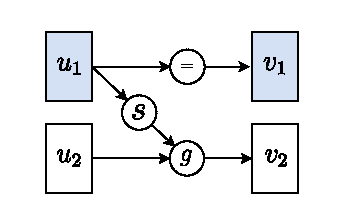
\includegraphics{figures/NICE.pdf}
        \caption[NICE Architecture]{ The architecture of a \ac{NICE} layer. $s$ is a neural network, and $g$ is an affine function.}
        \label{fig:nice}
    \end{subfigure}
    \hspace{0.02\textwidth}
    \begin{subfigure}{0.5\textwidth}
        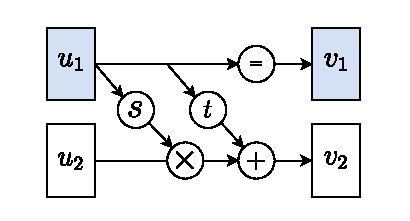
\includegraphics{figures/RealNVP.pdf}
        \caption[RealNVP Architecture]{ The architecture of a \ac{RealNVP} layer. $s$ and $t$ are neural networks. The symbol $\times$ stands for element-wise product by the exponential function over input.}
        \label{fig:realnvp}
    \end{subfigure}
    \begin{subfigure}{\textwidth}
        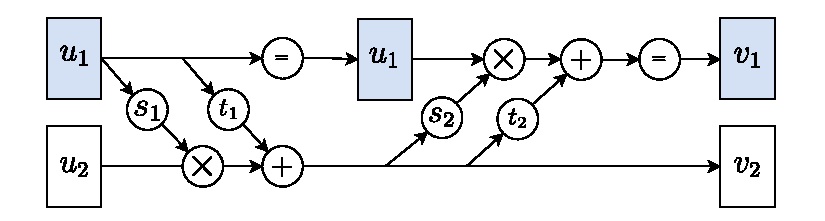
\includegraphics{figures/INN.pdf}
        \caption[INN Architecture]{ The architecture of an \ac{INN} layer. $s_1$, $s_2$, $t_1$, and $t_2$ are neural networks. The symbol $\times$ stands for element-wise product by the exponential function over input.}
        \label{fig:inn}
    \end{subfigure}
    \caption[Coupling Flow Architecture]{ The architectures of coupling flows. The input of the layer is $\boldsymbol{u}$ and the output is $\boldsymbol{v}$.}
    \label{fig:coupling}
\end{figure}

The first proposed coupling flow is \ac{NICE} \citep{dinh2015nice}. The input variables $\boldsymbol{u}$ are split into two parts $[\boldsymbol{u}_1, \boldsymbol{u}_2]$, and the corresponding output variables are $\boldsymbol{v} = [\boldsymbol{v}_1, \boldsymbol{v}_2]$. The architecture in the forward direction is formulated by the following functions:
\begin{equation}
    \boldsymbol{v}_1 = \boldsymbol{u}_1, \quad \boldsymbol{v}_2 = g(\boldsymbol{u}_2;s(\boldsymbol{u}_1)),
\end{equation}
where $s$ is a neural network and $g$ is an affine function $g(a;b)=a+b$ or $a\odot b$. The forward architecture is illustrated in Figure~\ref{fig:nice}.
Then, the inverse functions are easily calculated:
\begin{equation}
    \boldsymbol{u}_1 = \boldsymbol{v}_1,\quad \boldsymbol{u}_2 = g^{-1}(\boldsymbol{v}_2;s(\boldsymbol{u}_1)).
\end{equation}
From the above functions, the Jacobian matrix is:
\begin{equation}
\frac {\partial \boldsymbol{v}}{\partial \boldsymbol{u}}=\begin{bmatrix}
\partial \boldsymbol{v}_1/\partial \boldsymbol{u}_1 & \partial \boldsymbol{v}_1/\partial \boldsymbol{u}_2 \\
\partial \boldsymbol{v}_2/\partial \boldsymbol{u}_1 & \partial \boldsymbol{v}_2/\partial \boldsymbol{u}_2\\
\end{bmatrix}=\begin{bmatrix}
\boldsymbol{I} & \boldsymbol{0} \\
\partial \boldsymbol{v}_2/\partial \boldsymbol{u}_1 & \partial g(\boldsymbol{u}_2;s(\boldsymbol{u}_1))/\partial \boldsymbol{u}_2\\
\end{bmatrix}
\end{equation}
Because of the triangle matrix, the determinant is $ \partial g(\boldsymbol{u}_2;s(\boldsymbol{u}_1))/\partial \boldsymbol{u}_2$.
By composing multiple coupling layers, we can construct increasingly complex hierarchical transformations. Since each coupling layer preserves a subset of its input unchanged, it is essential to alternate the roles of the partitioned subsets across successive layers. This ensures that all input dimensions are eventually processed. Analyzing the Jacobian reveals that a minimum of three coupling layers is required for full inter-dimensional interaction. In practice, we typically employ four layers to achieve sufficient expressiveness.

An improved architecture is \ac{RealNVP}, where one part of the variables is processed by two neural networks. The forward transformation is:
\begin{equation}
    \boldsymbol{v}_1 = \boldsymbol{u}_1, \quad \boldsymbol{v}_2 = \boldsymbol{u}_2\odot\exp(s(\boldsymbol{u}_1))+t(\boldsymbol{u}_1).
\end{equation}
And the inverse transformation is:
\begin{equation}
    \boldsymbol{u}_1 = \boldsymbol{v}_1, \quad \boldsymbol{u}_2 = (\boldsymbol{v}_2-t(\boldsymbol{u}_1))\odot\exp(-s(\boldsymbol{u}_1)).
\end{equation}
The Jacobian determinant $\det|\partial\boldsymbol{v}/\boldsymbol{u}|$ is then $\exp(\Sigma_i s(\boldsymbol{u}_{1,i}))$.
The architecture is shown in Figure~\ref{fig:realnvp}. To interact all variables in one block, \ac{INN} \citep{ardizzone2019inn} extends \ac{RealNVP} by another same coupling block, as shown in Figure~\ref{fig:inn}. 

A further enhancement of \ac{RealNVP} is Glow \citep{kingma2018glow}, which inserts an invertible normalization layer and an invertible permutation layer before affine transformation. \ac{HINT} \citep{kruse2021hint} partitions the inputs of coupling blocks recursively to construct a dense, triangular Jacobian. Another method to increase interaction among variables is \ac{MAF} \citep{papamakarios2018maf}, which can be considered as a generalized \ac{RealNVP} that leverages autoregressive transformations between variables. Apart from affine coupling, \ac{NSF} \citep{durkan2019neuralsplineflows} applies monotonic rational-quadratic spline functions, enabling more expressive and smooth transformations, however, at the cost of higher complexity. 

Such flows build step-wise invertible transformations between distributions, enabling tractable Jacobian calculation and density estimation. A notable drawback lies in the strict architectural constraint on coupling blocks. To release this limitation, residual flows \citep{behrmann2019ires, chen2020resflow} introduce invertible mapping through specified residual blocks. A residual block \citep{he2015residual} takes the form $f(x)=x+F(x)$, where $F$ is a neural network. When $F$ is constrained to be Lipschitz continuous and the Lipschitz constant is smaller than 1 (explained in \ref{sec:cnf}), the function $f(x)$ is invertible. The residual block can be seen as an Euler discretization of an \ac{ODE} \citep{lu2020finitelayer, ruthotto2018deep, haber2017stable}, which is the foundation of continuous \acp{NF}. 

\subsubsection{Continuous Flows}
When the transformation from latent space to data space is modeled by a continuous dynamical system, the \ac{NF} is called a continuous \ac{NF}. The continuous dynamical system can be formulated by a Neural \ac{ODE}, which is introduced as follows.
\label{sec:cnf}
\paragraph{Neural \acp{ODE}}
For a dynamical system with states $\boldsymbol{h}$, an \ac{ODE} is:
\begin{equation}
    \frac{d\boldsymbol{h}(t)}{dt} = f(\boldsymbol{h}(t), t; \boldsymbol{\theta}),
\end{equation}
where $\boldsymbol{\theta}$ denotes system parameters. When the \ac{ODE} is modeled by neural networks, it becomes a Neural \ac{ODE} \citep{chen2019node}. Given the initial state $\boldsymbol{h}(0)$, the final state $\boldsymbol{h}(T)$ is the solution of the initial value problem at the time step $T$ using a numerical solver. The loss function of training a Neural \ac{ODE} is:
\begin{equation}
    L(\boldsymbol{h}(T))=L(\int_0^Tf(\boldsymbol{h}(t), t; \boldsymbol{\theta})dt),
\end{equation}
where $f$ is a neural network parameterized by $\boldsymbol{\theta}$.
A straightforward application of Neural \acp{ODE} is learning continuous time-series models. Moreover, when the time step is interpreted as architectural depth, the distributional transformation in \acp{NF} can also be constructed with a Neural \ac{ODE}. The Neural \ac{ODE} replaces an infinite number of transformations by change of variables with a single neural network, which represents the derivative of transformation at each depth. This enables more efficient and expressive probabilistic modeling and inference.

A central technical challenge in training continuous-depth networks lies in executing reverse-mode differentiation (commonly known as backpropagation) through the ODE solver. This process requires computing gradients with respect to network parameters at various time points backwards from $t=T$ to $t=0$, resulting in large memory cost to store the intermediate states. The solution is using the adjoint method \citep{Bittner1963, adjoint1963}. The principle of the adjoint method is to solve a backward \ac{ODE} alongside the forward \ac{ODE} whenever intermediate states are required. Compared to storing all intermediate states of the forward \ac{ODE}, the adjoint method reduces memory cost at the expense of increased computational cost. This trade-off makes it more suitable for long sequences and high-dimensional variables, but less efficient for computationally complex network architectures.

% Denoting an adjoint state as $\boldsymbol{a}(t)=\partial L/\partial\boldsymbol{h}(t)$, the new \ac{ODE} problem to solve is:
% \begin{equation}
%     \begin{cases}
% \frac{\partial \boldsymbol{a}(t)}{\partial t}=-\boldsymbol{a}^T(t)\partial f(\boldsymbol{h}(t),t,\boldsymbol{\theta})/\partial \boldsymbol{h}(t), \\
% \frac{d\boldsymbol{h}(t)}{dt} = f(\boldsymbol{h}(t), t, \boldsymbol{\theta}).
% \end{cases}
% \end{equation}

\paragraph{Lipschitz continuity}
We define a continuous \ac{NF} as a Neural \ac{ODE}:
\begin{equation}
    \label{eq:cnfode}
    \frac{d\boldsymbol{z}(t)}{dt}=f(\boldsymbol{z},t;\boldsymbol{\theta}),
\end{equation}
where $\boldsymbol{z}(t)$ follows the density $p(\boldsymbol{z}(t))$ at an instantaneous step $t\in[t_0, t_1]$. The \ac{NF} $f$ is parameterized by $\boldsymbol{\theta}$.
To apply the Neural \ac{ODE} as continuous \acp{NF}, the function $f$ should be uniformly Lipschitz continuous in the states $\boldsymbol{z}(t)$ and continuous in depth $t$. 

The definition of a Lipschitz continuous function is referred to the work by \citeauthor{khromov2024Lipschitz} \citeyearpar{khromov2024Lipschitz}.
\begin{definition}
(\textbf{Lipschitz continuous function}) A function $f:\mathbb{R}^d\rightarrow\mathbb{R}^K$, defined on some domain $dom(f)\subseteq \mathbb{R}^d$, is called $C$-Lipschitz continuous w.r.t. some $\alpha$-norm, if $\forall \boldsymbol{x}, \boldsymbol{y} \in dom(f):\left\| f(\boldsymbol{x})-f(\boldsymbol{y})\right\|_{\alpha}\leq C\left\| \boldsymbol{x}-\boldsymbol{y}\right\|_{\alpha}$. $C$ is called Lipschitz constant of $f$ and $0<C<\inf$.
\end{definition}

The Lipschitz condition guarantees that there exists a unique solution curve $\boldsymbol{t}$ for every initial condition $\boldsymbol{z}(0)$. This is known as the Picard–Lindel\"of theorem. Assuming the dynamics function $f$ is smooth, then it is a diffeomorphism, which means we also get the same $\boldsymbol{z}(0)$ by running the \ac{ODE} backwards. Recalling the residual flows, where the Lipschitz constant must be smaller than 1, invertibility is ensured naturally by a smooth and Lipschitz continuous \ac{ODE}. In practice, neural networks with smooth continuous activation functions satisfy this requirement.

\paragraph{Continuous \acp{NF}}
Besides for the ODE \ref{eq:cnfode}, the log-density of states changes according to another \ac{ODE}, the instantaneous change-of-variables formula \citep{chen2019node}:
\begin{equation}
    \label{eq:instchangeofvar}
    \frac{\partial\log p(\boldsymbol{z}(t))}{\partial t}=-\text{Tr}(\frac{\partial f(\boldsymbol{z}(t),t;\boldsymbol{\theta})}{\partial\boldsymbol{z}(t)}).
\end{equation}
The trace can be approximated through Skilling-Hutchinson trace estimator \citep{Skilling1989,Hutchinson01011990,adams2018adams}:
\begin{equation}
    \text{Tr}(\frac{\partial f}{\partial \boldsymbol{z}(t)})=\mathbb{E}_{p(\boldsymbol{\epsilon})}[\boldsymbol{\epsilon}^T\frac{\partial f}{\partial \boldsymbol{z}(t)}\boldsymbol{\epsilon}],
\end{equation}
where $\boldsymbol{\epsilon}$ is a noise vector sampled from a standard normal distribution and kept unchanged to maintain determinism of the \ac{ODE}. The part of vector-Jacobian product $\boldsymbol{\epsilon}^T\partial f/\partial \boldsymbol{z}(t)$ is computed with automatic differentiation.

For a continuous \ac{NF} between the data distribution $p(\boldsymbol{x})=p(\boldsymbol{z}(t_1))$ and the latent distribution $p_{Z_0}(\boldsymbol{z}_0)=p(\boldsymbol{z}(t_0))=\mathcal{N}(\boldsymbol{0}, \boldsymbol{I})$, we define the augmented states as $[\boldsymbol{z}(t), \log p(\boldsymbol{x})-\log p(\boldsymbol{z}(t))]$.
Then, building the continuous \ac{NF} is equivalent to solving the initial value problem \citep{grathwohl2018ffjord}:
\begin{equation}
    \underbrace{\begin{bmatrix}
\boldsymbol{z}_0 \\
\log p(\boldsymbol{x}) - \log p_{Z_0}(\boldsymbol{z}_0)
\end{bmatrix}}_{\text{solutions}}
=
\int_{t_1}^{t_0}
\underbrace{\begin{bmatrix}
f(\boldsymbol{z}(t), t; \theta) \\
-\text{Tr}\left(\frac{\partial f}{\partial \boldsymbol{z}(t)}\right)
\end{bmatrix}}_{\text{dynamics}} dt,
\underbrace{\begin{bmatrix}
\boldsymbol{z}(t_1) \\
\log p(\boldsymbol{x}) - \log p(\boldsymbol{z}(t_1))
\end{bmatrix}}_{\text{initial values}}
=
\begin{bmatrix}
\boldsymbol{x} \\
0
\end{bmatrix}.
\end{equation}
It is worth noting that the integral is backwards calculated from $t_1$ to $t_0$, meaning from the data side to the latent side. The time span can also be optimized to further improve the computational efficiency \citep{du2022toflow}.

Continuous \acp{NF} release the architectural constraints of discrete flows, allowing more flexible and expressive density estimation through the integration of Neural \acp{ODE}. This improved expressiveness, however, comes at a cost: computing the Jacobian trace and the associated ODE integrals is significantly more expensive than in stacked coupling flows.

\subsubsection{Flow Matching}
\label{sec:flowmatching}
\ac{FM} \citep{lipman2023flowmatching} is a novel approach for training continuous \acp{NF}. The key idea is to learn a vector field that directly matches the step-by-step transport (infinitesimal transport) between the data distribution and the latent distribution. This is achieved by minimizing the expected squared error between the learned vector field and the true velocity field defined by the optimal transport plan. The optimal transport plan is normally a linear interpolation between the latent samples $\boldsymbol{z}(t_0)$ and the data samples $\boldsymbol{x}=\boldsymbol{z}(t_1)$:
\begin{equation}
    \boldsymbol{v}^{OT}(\boldsymbol{z}, t) = \frac{\boldsymbol{z}(t_1)-\boldsymbol{z}(t_0)}{t_1 - t_0}.
\end{equation}
The training objective is formulated as:
\begin{equation}
    L(\boldsymbol{\theta}) = \mathbb{E}_{t\sim\mathcal{U}(0,1),\boldsymbol{z}\sim p_t(\boldsymbol{z})}\left[\left\|v_{\boldsymbol{\theta}}(\boldsymbol{z}, t; \boldsymbol{\theta}) - \boldsymbol{v}^*(\boldsymbol{z}, t)\right\|^2\right],
\end{equation}
where $v_{\boldsymbol{\theta}}(\boldsymbol{z}, t; \boldsymbol{\theta})$ is the learned vector field parameterized by $\boldsymbol{\theta}$, and $\boldsymbol{v}^*(\boldsymbol{z}, t)$ is the true velocity field derived from the optimal transport plan. Simply put, the \ac{FM} loss regresses the vector field $\boldsymbol{v}^*$ with a neural network $v_{\boldsymbol{\theta}}$. Upon reaching zero loss, the learned continuous \ac{NF} model will generate data samples by integrating the learned vector field from $t_0$ to $t_1$. 

The main difference from other \acp{NF} is that \ac{FM} is not trained by maximizing likelihood via change of variables between distributions. Instead, it focuses on learning the vector field that defines the continuous transformation between distributions. This approach avoids the computational overhead of solving \acp{ODE} during training, making it more efficient and scalable to high-dimensional data. On the other hand, \ac{FM} cannot be directly applied to exact density estimation because it does not transform the data distribution into a known latent distribution. The sample density it generates is only an approximation of the data density. For exact estimation, \ac{FM} must invert the generative process via a backward \ac{ODE}, which makes it computationally heavier than the single-pass inference of other \acp{NF}.

\subsubsection{Conditional Normalizing Flows}
\label{sec:condnf}
Such capabilities of estimating complex densities are desirable in Bayesian inference of the posterior distribution of variables given observations $p(\boldsymbol{x}|\boldsymbol{y})$. Similar to \ac{VAE}, amortized Bayesian inference \citep{radev2021diss} is applied in \ac{NF} to achieve a general posterior estimation across all data points. Obtaining the posterior distribution is represented by a conditional density transformation via a \ac{CNF}. The change of variables for a \ac{CNF} extends the standard one (\ref{eq:xnfz}) by the condition $\boldsymbol{y}$:
\begin{equation}
    p_{X|Y}(\boldsymbol{x}|\boldsymbol{y}) = p_{Z|Y}(f^{-1}(\boldsymbol{x},\boldsymbol{y})|\boldsymbol{y})\det\left|\frac{\partial f^{-1}(\boldsymbol{x},\boldsymbol{y})}{\partial\boldsymbol{x}}\right|,
\end{equation}
where the mapping $f:Z\rightarrow X\times Y$ is bijective between $X$ and $Z$, and $\boldsymbol{z}=f^{-1}(\boldsymbol{x},\boldsymbol{y})$.

Designing such a \ac{CNF} requires addressing two key considerations in advance: (1) how to manage the conditioned latent variables, and (2) how to incorporate conditions into the flow architecture while preserving invertibility. \citeauthor{winkler2023cnf} \citeyearpar{winkler2023cnf} proposed to build the conditional prior $p_{Z|Y}(\boldsymbol{z}|\boldsymbol{y})$ as a diagonal Gaussian:
\begin{equation}
    p_{Z|Y}(\boldsymbol{z}|\boldsymbol{y}) = \mathcal{N}{\boldsymbol{z}|\mu(\boldsymbol{y}, \text{diag}(\sigma^2(\boldsymbol{y})))}.
\end{equation}
For simpler conditioning scenarios, incorporating the conditional prior could accelerate the transformation through leveraging the information from conditions. For complex conditions, summarizing the conditions through mean and variance may result in information loss, thereby degrading posterior estimation quality. This limitation likely explains why most existing work on \acp{CNF} adopts a standard Gaussian as the latent base distribution, bypassing the need for an explicitly conditioned prior and relying instead on the normalizing flows to capture conditional information.

In terms of architectures of \acp{CNF}, a direct adaptation based on the \ac{INN} is the \ac{cINN} \citep{ardizzone2019cinn}. It takes the condition as augmented input to the neural networks. In cases of higher-dimensional conditions, such as images, \citeauthor{govinda2021cinn} \citeyearpar{govinda2021cinn} apply a staged \ac{cINN} coupled with a staged condition network, wherein the conditions are progressively processed, and each intermediate representation is fed into its corresponding \ac{cINN} block.

In scenarios involving complex conditions and relatively simple target variables, BayesFlow \citep{radev2020bayesflow} offers a general framework by extracting informative representations through a summary network and incorporating them, alongside the inputs, as augmented inputs to the \ac{cINN}. This framework is particularly well-suited for parameter identification from time series observations, where the summary network is typically chosen as a time series modeling architecture, such as \ac{RNN}. The architecture is illustrated in Figure~\ref{fig:bayesflow}. Both the summary network and \ac{cINN} are optimized together by minimizing the \ac{KL}-divergence between the true posterior density and the estimated one (similar to Equation \ref{eq:kl_nf}):
\begin{multline}
\label{eq:kl_cnf}
D_{\text{KL}}(p_{X|Y}(\boldsymbol{x}|\boldsymbol{y})||p_{X|Y}(\boldsymbol{x}|\boldsymbol{y};\boldsymbol{\theta},\boldsymbol{\phi}))\approx const. - \\
\frac{1}{M}\sum_{m=1}^{M}[\log p_{Z}(f_{\boldsymbol{\theta}}^{-1}(\boldsymbol{x}^{(m)}, h_{\boldsymbol{\phi}}(\boldsymbol{x}^{(m)})))+\log\det\left|\boldsymbol{J}_{f_{\boldsymbol{\theta}}^{-1}}(\boldsymbol{x}^{(m)},h_{\boldsymbol{\phi}}(\boldsymbol{x}^{(m)}))\right|],
\end{multline}
where $f$ is the \ac{cINN} parameterized by $\boldsymbol{\theta}$ and $h$ is the summary network parameterized by $\boldsymbol{\phi}$.

\begin{figure}[htp!]
    \centering
    \includegraphics[width=0.85\textwidth]{figures/BayesFlow.pdf}
    \caption[BayesFlow Architecture]{ The architecture of BayesFlow. The blue arrows indicate the forward direction for training BayesFlow, while the yellow arrows indicate the reverse direction for inference. The summary network extracts informative representations from the observations, which are then fed into the \ac{cINN} alongside the target variables.}
    \label{fig:bayesflow}
\end{figure}
The joint optimization approach encourages the summary network to deliver maximally useful information to the \ac{cINN} thus improve the inference capability. In this work, we adopt the BayesFlow framework as a flexible and scalable solution for amortized Bayesian inference, adapting its summary network to accommodate diverse time series observations. This framework forms the foundation of our proposed methods for parameter identification, system dynamics modeling, and state estimation.

\subsection{From Bayesian Inference to Control}
This section bridges the Bayesian inference methodologies discussed above to their practical applications in control systems. We first review how Bayesian approaches are employed for system identification and state estimation. Next, we introduce \acf{MPC}, which is a widely used model-based control technique for optimal decision-making based on the system identification results. Finally, we discuss \acf{RL} as a data-driven control paradigm, highlighting its ability to learn control policies directly from interactions with the environment without requiring explicit system models. Together, these approaches illustrate the synergy between Bayesian inference and modern control strategies, enabling robust and adaptive solutions for complex dynamical systems.

\subsubsection{Bayesian System Identification}
An essential goal of system modeling and identification is to provide a rigorous framework for predicting and controlling the future evolution of system outputs. For any control strategy, the decision-maker needs to predict how the system will behave under any possible control input. This requires access to the joint probability distribution of the future input-output sequence, which can be factorized using the chain rule of probability \citep{BayesSysId1981}:
\begin{equation}
    p(\mathcal{D}_{(t_1:t_N)}|\mathcal{D}_{t_0})=\prod _{n=1}^{N}p(\boldsymbol{y}_{t_n}|\boldsymbol{u}_{t_n}, \mathcal{D}_{t_{n-1}})p(\boldsymbol{u}_{t_n}|\mathcal{D}_{t_{n-1}}),
\end{equation}
where $\mathcal{D}_{t_n}$ denotes the input-output pair at the time step $t_n$, i.e., $\mathcal{D}_{t_n}=\{\boldsymbol{u}_{t_n}, \boldsymbol{y}_{t_n}\}$.
The conditional probability density $p(\boldsymbol{u}_{t_n}|\mathcal{D}_{t_{n-1}})$ describes the process of determining the input $\boldsymbol{u}_{t_n}$ on the basis of the known past history. The left part $p(\boldsymbol{y}_{t_n}|\boldsymbol{u}_{t_n}, \mathcal{D}_{t_{n-1}})$ represents the dependence of the output on the corresponding input and the known past history, which can be interpreted as a system model or function to predict output with given control input. Identifying this system consists of two steps: model selection and parameter identification. The process of finding the most plausible model from a group of candidates is model selection. Then, system identification focuses on inferring parameters of a chosen system model.
\paragraph{Bayesian model selection}
Among different model structures $\{\mathcal{M}_i\}$, $i=1,\ldots,|\mathcal{M}|$, the probability density of the model $\mathcal{M}_i$ given the data $\mathcal{D}$ measures whether the model is suitable for the dataset, which can also be written using Bayes’ theorem:
\begin{equation}
    p(\mathcal{M}_i|\mathcal{D})=\frac{p(\mathcal{D}|\mathcal{M}_i)p(\mathcal{M}_i)}{p(\mathcal{D})}.
\end{equation}
Model selection is also as known as model comparison. The relative probability density of two different models given same data $\mathcal{D}$ is:
\begin{equation}
    \frac{p(\mathcal{M}_i|\mathcal{D})}{p(\mathcal{M}_j|\mathcal{D})} = \frac{p(\mathcal{D}|\mathcal{M}_i)p(\mathcal{M}_i)}{p(\mathcal{D}|\mathcal{M}_j)p(\mathcal{M}_j)}.
\end{equation}
Since a model has multiple undetermined parameters, the distribution $p(\mathcal{D}|\mathcal{M})$ is obtained by integral of all variants of parameters. The integral is usually untractable. Instead, \ac{DIC} \citep{Spiegelhalter2002,Spiegelhalter2014, li2025DIC} is applied as the model selection criterion. A deviance is defined as follows:
\begin{equation}
    \text{dev}(\boldsymbol{\theta}) = -2\log p(\mathcal{D}|\boldsymbol{\theta}, \mathcal{M}),
\end{equation}
where $\boldsymbol{\theta}$ denotes the parameters of the model $\mathcal{M}$. Then, the \ac{DIC} is defined as:
\begin{equation}
    \text{DIC}(\mathcal{M}) = \mathbb{E}_{\mathcal{M}}[\text{dev}(\boldsymbol{\theta})] + P_D(\mathcal{M}),
\end{equation}
where the first term is interpreted as a Bayesian measure of model fit:
    \begin{equation}
        \mathbb{E}_{\mathcal{M}}[\text{dev}(\boldsymbol{\theta})] = \int p(\boldsymbol{\theta}|\mathcal{D}, \mathcal{M})\text{dev}(\boldsymbol{\theta})d\boldsymbol{\theta},
    \end{equation}
and the second term is used to measure the model complexity:
    \begin{equation}
        P_D(\mathcal{M}) = \mathbb{E}_{\mathcal{M}}[\text{dev}(\boldsymbol{\theta})] - \text{dev}(\overline{\boldsymbol{\theta}}),\quad \overline{\boldsymbol{\theta}}=\int p(\boldsymbol{\theta}|\mathcal{D},\mathcal{M})\boldsymbol{\theta}d\boldsymbol{\theta}.
    \end{equation}
The posterior $p(\boldsymbol{\theta}|\mathcal{D},\mathcal{M})$ is obtained by \ac{MCMC}.
\ac{DIC} balances the goodness of fit (how well the model explains the data) and the model complexity (the number of parameters in the model). A lower \ac{DIC} value indicates better model fit for the given dataset. 

\paragraph{Bayesian Parameter Identification}
We first define a chosen system model with unknown parameters $\boldsymbol{\theta}$:
\begin{equation}
    \boldsymbol{y}_t=f(\boldsymbol{u}_t, \boldsymbol{\theta})+\boldsymbol{\epsilon}_t.
\end{equation}
The optimal parameters are selected by \ac{MAP} estimation:
\begin{equation}
    \boldsymbol{\theta}^*_{MAP}=\arg \max_{\boldsymbol{\theta}}p(\boldsymbol{\theta}|\mathcal{D}).
\end{equation}
Applying Bayes' rule (\ref{eq:bayes}), it becomes:
\begin{equation}
    \boldsymbol{\theta}^*_{MAP}=\arg \max_{\boldsymbol{\theta}}[\prod_{\{\boldsymbol{u}_i,\boldsymbol{y}_i\}\in\mathcal{D}} p(\boldsymbol{y}_i|\boldsymbol{u}_i,\boldsymbol{\theta})]p(\boldsymbol{\theta}),
\end{equation}
where $p(\mathcal{D})$ is dropped off since it is a constant with respect to $\boldsymbol{\theta}$. The noise $\boldsymbol{\epsilon}_t$ is commonly assumed to be Gaussian. Thus, the distribution $p(\boldsymbol{y}_i|\boldsymbol{u}_i,\boldsymbol{\theta})$ has a closed form, which makes this term equivalent to a weighted mean squared error. The term of the prior density $p(\boldsymbol{\theta})$ performs as $L2$ regularization.
On top of the estimate of parameters, the confidence interval of parameters can also be obtained from the posterior distribution.

\subsubsection{Bayesian State Estimation}
Applying the estimated posterior of system parameters again as a prior, and updating the posterior with new data, this is the basic idea of Bayesian state estimation \citep{bayesestimation}. State estimation involves inference of the internal system states, which are not directly measurable. Expressing the state estimation problem in a probabilistic framework, the goal is to infer the posterior distribution of the states given observations $p(\boldsymbol{x}_{0:t}|\boldsymbol{y}_{1:t})$. Assuming a Markovian system, the posterior of the state chain is factorized as:
\begin{equation}
    \begin{split}
        p(\boldsymbol{x}_{0:t}|\boldsymbol{y}_{1:t})=p(\boldsymbol{x}_{0:t}|\boldsymbol{y}_{t}, \boldsymbol{y}_{1:t-1})&=\frac{p(\boldsymbol{y}_t|\boldsymbol{x}_{0:t}, \boldsymbol{y}_{1:t-1})p(\boldsymbol{x}_{0:t}|\boldsymbol{y}_{1:t-1})}{p(\boldsymbol{y}_t|\boldsymbol{y}_{1:t-1})} \quad\text{[Bayes' rule]} \\
        &=\frac{p(\boldsymbol{y}_t|\boldsymbol{x}_t)p(\boldsymbol{x}_{0:t}|\boldsymbol{y}_{1:t-1})}{p(\boldsymbol{y}_t|\boldsymbol{y}_{1:t-1})} \quad\text{[Markov property]} \\
        &=\frac{p(\boldsymbol{y}_t|\boldsymbol{x}_t)p(\boldsymbol{x}_{t}|\boldsymbol{x}_{t-1})}{p(\boldsymbol{y}_t|\boldsymbol{y}_{1:t-1})}p(\boldsymbol{x}_{0:t-1}|\boldsymbol{y}_{1:t-1}),
    \end{split}
\end{equation}
where $p(\boldsymbol{x}_{t}|\boldsymbol{x}_{t-1})$ is referred as evolution model, or state transition model, and $p(\boldsymbol{y}_t|\boldsymbol{x}_t)$ is called observation model, or measurement model. The posterior $p(\boldsymbol{x}_{0:t-1}|\boldsymbol{y}_{1:t-1})$ is the result of the previous time step. The equation above describes a recursive process of state estimation.
\paragraph{Bayesian Filters}
\label{sec:bayesfilter}
Considering only one state $\boldsymbol{x}_{t}$ at a time, the problem is called marginal state estimation, or filtering. The equation becomes:
\begin{equation}
    \label{eq:bayesfilter}
    \begin{split}
        p(\boldsymbol{x}_{t}|\boldsymbol{y}_{1:t})&=\frac{p(\boldsymbol{y}_t|\boldsymbol{x}_t)p(\boldsymbol{x}_{t}|\boldsymbol{y}_{1:t-1})}{p(\boldsymbol{y}_t|\boldsymbol{y}_{1:t-1})}\\
        &=\frac{p(\boldsymbol{y}_t|\boldsymbol{x}_t)}{p(\boldsymbol{y}_t|\boldsymbol{y}_{1:t-1})}\int p(\boldsymbol{x}_{t}|\boldsymbol{x}_{t-1})p(\boldsymbol{x}_{t-1}|\boldsymbol{y}_{1:t-1})d\boldsymbol{x}_{t-1}.
    \end{split}
\end{equation}
Usually, calculation of the above equation is divided into two steps: prediction and update. In the prediction step, the result of state transition from $\boldsymbol{x}_{t-1}$ to $\boldsymbol{x}_t$ is computed through the evolution model. In the update step, the last observation likelihood $p(\boldsymbol{y}_t|\boldsymbol{x}_t)$ weights the predicted belief. These two steps build the Bayesian filtering methods: Kalman filters and particle filters \citep{chen_bayesian_2003}.

The \ac{KF} \citep{kf1960} can be directly derived from Equation \ref{eq:bayesfilter} under the assumptions of linear systems and Gaussian noise. For a linear system:
\begin{subequations}
    \begin{align}
        \boldsymbol{x}_t &= F_t\boldsymbol{x}_{t-1} + \boldsymbol{w}_t, \quad \boldsymbol{w}_t\sim\mathcal{N}(\boldsymbol{0}, \Sigma_{w_t}),\\
        \boldsymbol{y}_t &= H_t\boldsymbol{x}_t + \boldsymbol{v}_t, \quad \boldsymbol{v}_t\sim\mathcal{N}(\boldsymbol{0}, \Sigma_{v_t}),
    \end{align}
\end{subequations}
the iterative algorithm of filtering is:
\begin{itemize}
    \item Prediction:
    \begin{subequations}\label{eq:kalman_prediction}
    \begin{align}
        \boldsymbol{x}'_t &= F_t\boldsymbol{x}_{t-1}, \label{eq:kalman_prediction_a} \\
        \Sigma'_{t} &= F_t\Sigma_{t-1}F_t^T+\Sigma_{w_t}. \label{eq:kalman_prediction_b}
    \end{align}
    \end{subequations}
    \item Update:
    \begin{subequations}\label{eq:kalman_update}
    \begin{align}
        K_t &= \Sigma'_{t}H_t^T(H_t\Sigma'_{t}H_t^T+\Sigma_{v_t})^{-1} \label{eq:kalman_update_a}, \\
        \boldsymbol{x}_t &= \boldsymbol{x}'_t+K_t(\boldsymbol{y}_t-H_t\boldsymbol{x}'_t) \label{eq:kalman_update_b}, \\
        \Sigma_t &= (I-K_tH_t)\Sigma'_{t} \label{eq:kalman_update_c}.
    \end{align}
    \end{subequations}
\end{itemize}

For nonlinear systems, the \acf{EKF} \citep{simon2006optimal} obtains the matrices $F_t$ and $H_t$ by linearizing the nonlinear functions at the current estimate, i.e., $F_t=\nabla_{\boldsymbol{x}} f_t|_{\boldsymbol{x}_t}$ and $H_t=\nabla_{\boldsymbol{x}} h_t|_{\boldsymbol{x}_t}$. In such a way, the \ac{EKF} can be considered as the first-order approximation to the optimal terms. This approximation, however, can introduce large errors, which may lead to suboptimal performance and sometimes divergence of the filter. The \acf{UKF} \citep{ukf2000} addressed the approximation issues by carefully choosing a minimal set of samples points, which are called sigma points. The sigma points completely capture the mean and covariance of states, which are viewed as Gaussian random variables. The sample points are then propagated through the nonlinear functions, and the mean and covariance of the estimate are reconstructed from the transformed points. 

Relaxing the assumptions on model linearity and Gaussian noise, \ac{PF} \citep{pf1993, Elfring2021-xf} is a more general Bayesian filtering method. The integral in Equation \ref{eq:bayesfilter} is approximated through Monte Carlo estimation, yielding an average of all weighted particles. Each particle represents a possible state of the system, and its weight reflects the likelihood of that state given the observations. In the prediction step, each particle is propagated through the system dynamics. In the update step, weights are adjusted according to each particle based on the likelihood of the observation given the particle's state. Unlike Kalman filters, in each iteration of the \ac{PF}, a resampling step is included to avoid weight degeneracy, meaning that most particles carry very small weights over time. In the resampling step, particles are replaced with equally weighted ones, replicating high-weight particles and discarding low-weight ones.

In summary, \ac{KF} is efficient and provides optimal state estimates for linear systems with Gaussian noise. \ac{EKF} extends \ac{KF} to nonlinear systems through linearization, but may suffer from approximation errors. \ac{UKF}, instead of linearization, applies sigma points to better capture the mean and covariance of the state distribution, leading to more accurate estimates for highly nonlinear systems. \ac{PF} is the most flexible, capable of handling arbitrary nonlinearities and non-Gaussian noise, but computationally expensive due to the need for numerous particles.

\paragraph{State-Space Models}
For modeling system dynamics completely from data, \acfp{SSM} \citep{Durbin2012} are widely used. An \ac{SSM} consists of a latent state vector $\boldsymbol{x}_t$ and an observation vector $\boldsymbol{y}_t$. The state vector captures the internal dynamics of the system, while the observation vector represents the measurable outputs. $\boldsymbol{x}_t$ follows a Markov process, meaning that the previous state $\boldsymbol{x}_{t-1}$ carries all information to obtain the current state $\boldsymbol{x}_t$. $\boldsymbol{y}_t$ is solely dependent on the latent state $\boldsymbol{x}_t$. These assumptions lead to the following factorization of the joint distribution:
\begin{equation}
    p(\boldsymbol{y}_{1:T}, \boldsymbol{x}_{0:T}) = p(\boldsymbol{x}_0) \prod_{t=1}^{T}p(\boldsymbol{x}_t|\boldsymbol{x}_{t-1})p(\boldsymbol{y}_t|\boldsymbol{x}_t).
\end{equation}
In the simplest case, the state transition distribution $p(\boldsymbol{x}_t|\boldsymbol{x}_{t-1})$ and the observation distribution $p(\boldsymbol{y}_t|\boldsymbol{x}_t)$ are assumed to be linear Gaussian models:
\begin{subequations}
    \begin{gather}
        \boldsymbol{x}_0\sim\mathcal{N}(\boldsymbol{0}, \Sigma_0), \\
        \boldsymbol{x}_t=\boldsymbol{F}\boldsymbol{x}_{t-1}+\boldsymbol{w}_t, \quad \boldsymbol{w}_t\sim\mathcal{N}(\boldsymbol{0},\Sigma_{w_t})\\
        \boldsymbol{y}_t=\boldsymbol{H}\boldsymbol{x}_t+\boldsymbol{v}_t, \quad \boldsymbol{v}_t\sim\mathcal{N}(\boldsymbol{0},\Sigma_{v_t}).
    \end{gather}
\end{subequations}
In the previous section, we have shown estimation of states using Kalman filters with known system matrices ($\boldsymbol{F}$, $\boldsymbol{H}$) and noise covariance matrices ($\Sigma_{w_t}, \Sigma_{v_t}$). When these matrices are unknown, they can be estimated from data using the \ac{EM} algorithm \citep{Dempster1977}. The \ac{EM} algorithm iteratively maximizes the expected log-likelihood of the complete data (both observed and latent variables) given the current parameter estimates. The algorithm consists of two main steps:
\begin{itemize}
    \item E-step: Compute the expectations of the latent states using the current parameter estimates:
    \begin{equation*}
        E_t=E[\boldsymbol{x}_t],\quad E_{t,t}=E[\boldsymbol{x}_t\boldsymbol{x}_t^T],\quad E_{t,t-1}=E[\boldsymbol{x}_t\boldsymbol{x}_{t-1}^T].
    \end{equation*}
    The states come from running the Kalman filter (Equation \ref{eq:kalman_prediction}, \ref{eq:kalman_update}) on the current parameters.
    \item M-step: Update parameters using the expectations:
    \begin{subequations}
        \begin{align*}
            \boldsymbol{F}&=\left(\sum_{t=1}^{T}E_{t,t-1}\right)\left(\sum_{t=1}^{T}E_{t-1, t-1}\right)^{-1}, \quad \boldsymbol{H}=\left(\sum_{t=0}^{T}\boldsymbol{y}_tE_t^T\right)\left(\sum_{t=1}^{T}E_{t,t}\right)^{-1}, \\
            \Sigma_{w_t}&=\frac{1}{T}\left(\sum_{t=1}^{T}E_{t,t}-\boldsymbol{F}\sum_{t=1}^{T}E_{t,t-1}^T\right), \quad \Sigma_{v_t}=\frac{1}{T}\left(\sum_{t=0}^{T}\boldsymbol{y}_t\boldsymbol{y}_t^T-\boldsymbol{H}\sum_{t=0}^{T}\boldsymbol{y}_tE_t^T\right).
        \end{align*}
    \end{subequations}
\end{itemize}
The E-step and M-step are iterated until convergence. The \ac{EM} algorithm guarantees that the likelihood of the observed data does not decrease with each iteration, leading to convergence to a local maximum. Similar to Kalman filters, for nonlinear models, \acp{EKF} and \acp{UKF} are applied in the E-step; while for nonlinear and non-Gaussian \acp{SSM}, \acp{PF} are used to approximate the expectations in the E-step \citep{Durbin2000}.

\paragraph{Stochastic Differential Equations}
The core strength of \acp{SSM} lies in separating the latent states and noise, enabling capturing dynamics from the noisy observations. When we upgrade \acp{SSM} from discrete time to continuous time, \acfp{SDE} \citep{oksendal1985} are a natural choice for modeling the evolution of latent states. A general form of an \ac{SDE} is:
\begin{equation}
    dX_t = \mu(X_t, t)dt + \sigma(X_t, t)dW_t,
\end{equation}
where $dX_t$ is the infinitesimal change in the state, $\mu(X_t, t)$ is the drift function representing the deterministic part of the dynamics, $\sigma(X_t, t)$ is the diffusion function representing the stochastic part, and $W_t$ is a Wiener process (or Brownian motion) capturing the random fluctuations. A Wiener process is a standard stochastic process with independent, normally distributed increments and continuous paths. It has the following properties \citep{gabbiani2010mathematics}:
\begin{itemize}
    \item $W_0=0$.
    \item For any $0\leq s<t$, the increment $W_t-W_s$ is normally distributed with mean $0$ and variance $t-s$, i.e., $W_t-W_s\sim\mathcal{N}(0, (t-s)I)$.
    \item The process has independent increments, meaning that for any $0\leq t_0<t_1<\ldots<t_n$, the increments $W_{t_1}-W_{t_0}, W_{t_2}-W_{t_1}, \ldots, W_{t_n}-W_{t_{n-1}}$ are independent random variables.
\end{itemize}
A stochastic process is a collection of random variables indexed by time. It can be seen as a continuous-time generalization of the state vector in the \acp{SSM}. 

\subsubsection{Model Predictive Control}

\begin{figure*}[htp!]
    \centering
    \begin{subfigure}[b]{0.62\textwidth}
        \centering
        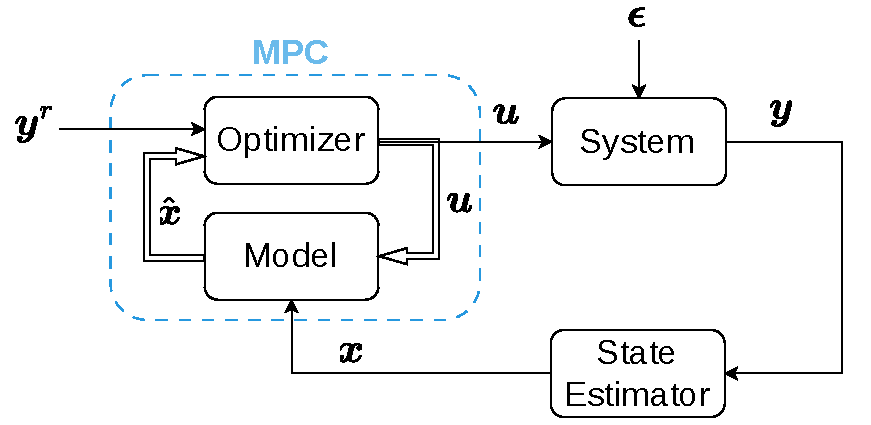
\includegraphics[width=\textwidth]{figures/MPC.pdf} 
        \caption[Schematic of Model Predictive Control]{Schematic of \ac{MPC} for a system with disturbance $\boldsymbol{\epsilon}$. This figure is adapted from \cite{Schwenzer2021}.}
        \label{fig:mpc}
    \end{subfigure}%
    ~ 
    \begin{subfigure}[b]{0.35\textwidth}
        \centering
        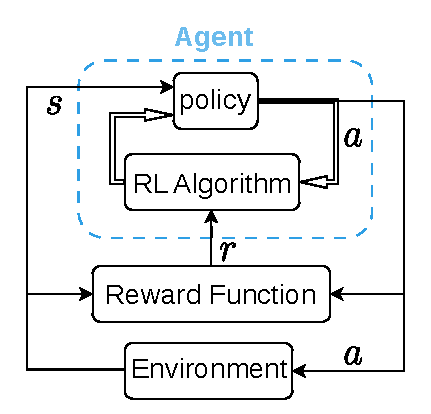
\includegraphics[width=\textwidth]{figures/RL.pdf} 
        \caption[Block diagram of Reinforcement Learning]{Block diagram of \ac{RL}. }
        \label{fig:rl}
    \end{subfigure}
    \caption{\ac{MPC} and \ac{RL}.}
\end{figure*}

After investigating Bayesian system identification and state estimation, we now turn our attention to control strategies, meaning optimizing system inputs given target and system observations. Control methods can be broadly categorized into model-based and model-free approaches. Model-based control relies on an explicit model of the system dynamics to predict future states and optimize control actions accordingly. In contrast, model-free control approaches do not require a state transition model of the system, instead learning control strategies directly from interactions with the system. A prominent example of model-based control is \acf{MPC} \citep{mpcreview1989, mpcbook2020}. 

\paragraph{Nominal Model Predictive Control}
A to-be-controlled system is at first modeled in discrete time steps:
\begin{subequations}
\begin{align}
    \label{eq:mpc_model}
    \boldsymbol{x}_{k+1} &= f(\boldsymbol{x}_k, \boldsymbol{u}_k), \\
    \boldsymbol{y}_k &= h(\boldsymbol{x}_k),
\end{align}
\end{subequations}
where $\boldsymbol{x}_k$ is the system state, $\boldsymbol{u}_k$ and $\boldsymbol{y}_k$ are the control input and system output at time step $k$, respectively. The function $f$ describes the state transition, and $h$ is the measurement function. Assuming that a full measurement or estimate of the state $\boldsymbol{x}_k$ is available, the objective of \ac{MPC} is to find an optimal sequence of control inputs $\boldsymbol{u}_{k:k+N-1}$ over a finite prediction horizon $N$. The objective function is:
\begin{subequations}
    \label{eq:mpc}
    \begin{gather}
        \min_{\boldsymbol{u}_{k:k+N-1}} \sum_{i=k}^{k+N-1}\ell(\boldsymbol{y}_{i}, \boldsymbol{u}_{i}, \boldsymbol{y}^r_{i})+L_f(\boldsymbol{y}^r_{k+N},\boldsymbol{y}_{k+N}),\\
        \ell(\boldsymbol{y}_{i}, \boldsymbol{u}_{i}, \boldsymbol{y}^r_{i})=(\boldsymbol{y}_{i}-\boldsymbol{y}^r_{i})^TQ_y(\boldsymbol{y}_{i}-\boldsymbol{y}^r_{i})+\boldsymbol{u}_{i}^TQ_u\boldsymbol{u}_{i},\\
        \text{subject to} \quad \boldsymbol{x}_{i+1} = f(\boldsymbol{x}_i, \boldsymbol{u}_i), \quad \boldsymbol{y}_i = h(\boldsymbol{x}_i),\\
        g_j(\boldsymbol{x}_i, \boldsymbol{u}_i)\leq 0, \quad j=1,\ldots,n_g, \quad i=k,\ldots,k+N-1,\\
        \boldsymbol{u}_{min}\leq\boldsymbol{u}_i\leq\boldsymbol{u}_{max}, \quad i=k,\ldots,k+N-1.
    \end{gather}
\end{subequations}
The cost function consists of a sum of stage costs $\ell$ and a final cost function $L_f$. In the stage cost, weighting matrices $Q_y$ and $Q_u$ are used to balance the trade-off between tracking performance and control effort. The reference trajectory $\boldsymbol{y}^r$ represents the desired output over the prediction horizon. The constraints $g_j(\boldsymbol{x}_i, \boldsymbol{u}_i)\leq 0$ can represent physical limitations of the system or other operational constraints. A simplified schematic of \ac{MPC} is shown in Figure~\ref{fig:mpc}. 

The optimization problem in \ac{MPC} can be solved using various numerical methods, such as sequential quadratic programming, interior-point methods, or gradient-based approaches \citep{Diehl2013}. The choice of method depends on the specific characteristics of the system model and constraints. The first step of the solution (Equation \ref{eq:mpc}) $\boldsymbol{u}^*_k$ is applied to the system, and the whole process is repeated at the next time step with updated state information. That's why \ac{MPC} is also known as receding horizon control \citep{Christophersen2007}.

\paragraph{Stochastic Model Predictive Control}
Taking system uncertainties and disturbances into account, robust \ac{MPC} \citep{rmpc1987} aims to satisfy system stability and constraints despite uncertainties and disturbances. There exist several sound robust \ac{MPC} methods, including Min-Max\ac{MPC} \citep{RAIMONDO20095}, scenario \ac{MPC} \citep{Calafiore_2013}, and stochastic \ac{MPC} \citep{HEIRUNG2018158,smpc2016}. The Min-Max \ac{MPC} chooses control actions that minimize the worst possible cost under bounded disturbances. The scenario \ac{MPC} samples a finite number of random uncertainty realizations as scenarios and optimizes control actions that satisfy constraints for each scenario. Stochastic \ac{MPC} incorporates the probabilistic descriptions of uncertainties into a stochastic optimal control problem through defining chance constraints. A mathematical formulation of stochastic \ac{MPC} is as follows \citep{HEIRUNG2018158} :
\begin{subequations}
    \label{eq:smpc}
    \begin{gather}
        \min_{\boldsymbol{u}_{k:k+N-1}}\sum_{i=k}^{k+N-1}\mathbb{E}[\ell(\boldsymbol{y}_{i}, \boldsymbol{u}_{i}, \boldsymbol{y}^r_{i})]+\mathbb{E}[L_f(\boldsymbol{y}^r_{k+N},\boldsymbol{y}_{k+N})],\\
        \text{subject to} \quad \boldsymbol{x}_{i+1} = f(\boldsymbol{x}_i, \boldsymbol{u}_i, \boldsymbol{w}_i), \quad \boldsymbol{y}_i = h(\boldsymbol{x}_i, \boldsymbol{v}_i),\\
        \mathbb{P}[g_j(\boldsymbol{x}_i, \boldsymbol{u}_i)\leq 0]\geq1-\beta_j, \quad\beta_j\in(0,1],\quad j=1,\ldots,n_g, \quad i=k,\ldots,k+N-1,\\
        \boldsymbol{u}_{min}\leq\boldsymbol{u}_i\leq\boldsymbol{u}_{max}, \quad i=k,\ldots,k+N-1.
    \end{gather}    
\end{subequations}   
The chance constraints $\mathbb{P}$ regularize the inequality constraints $g_i$, allowing for a small probability $\beta_j$ of constraint violation. The expectation in the cost function can be approximated using Monte Carlo simulation or analytical methods if the distributions are known.                                                                                                                                                                              
\subsubsection{Reinforcement Learning for Control}
When an accurate model of the system is unavailable or difficult to obtain, model-free control methods can be employed. Classical model-free control methods are \ac{PID} controllers \citep{Fliess_2013}. In recent years, data-driven control methods attract increasing attention. Especially, \acf{RL} can be viewed as a model-free framework for solving optimal control problems, and has been successfully applied in various domains, including robotics, game playing, and autonomous systems.

We first introduce the terminology of \ac{RL}:
\begin{itemize}
\item agent: the controller,
\item environment: the to-be-controlled system,
\item action: the control input, $a_t$,
\item state: the complete state of the environment, $s_t$,
\item policy: the control strategy, which can be deterministic ($a_t=\mu(s_t)$) or probabilistic ($a_t=\pi(\cdot|s_t)$),
\item reward: the feedback on the agent's success, $r_t=R(s_t,a_t)$.
\end{itemize}
The foundation of \ac{RL} is the \ac{MDP} \citep{mdp2014}. An \ac{MDP} is defined by the tuple $(\mathcal{S}, \mathcal{A}, P, R, \gamma)$, where $\mathcal{S}$ is the set of states, $\mathcal{A}$ is the set of actions, $P(s_{t+1}|s_t,a_t)$ is the state transition probability, $R(s_t,a_t)$ is the reward function, and $\gamma\in[0,1]$ is the discount factor. The interaction process between the agent and the environment at each time step $t$ is as follows: the agent observes the current state $s_t$, selects an action $a_t$ according to its policy $\pi(a_t|s_t)$, receives a reward $r_t=R(s_t,a_t)$ from the environment, and transitions to a new state $s_{t+1}$ based on the state transition probability $P(s_{t+1}|s_t,a_t)$. The goal of the agent is to learn an optimal policy $\pi^*$ that maximizes the expected cumulative discounted reward (known as value function):
\begin{equation}
    \pi^* = \arg\max_{\pi} \mathbb{E}{\pi}\left[\sum_{t=0}^{\infty} \gamma^t r_t\right].
\end{equation}          

In comparison to other optimal control methods, \ac{RL} methods aim to optimize long-term sequential decision-making performance. Besides, generality and scalability are the two main advantages of \ac{RL} methods. They can handle nonlinear, high-dimensional, and stochastic dynamics and also non-quadratic reward functions. The work by \citeauthor{rlforcontrol2018} \citeyearpar{rlforcontrol2018} provides a comprehensive review of \ac{RL} for control. 

It is worth noting that there is also an \ac{RL} method applying a surrogate model for the sake of improving the policy, which is called model-based \ac{RL} \citep{sutton1990, mbrl2020}. The surrogate model is learned from data in advance. Then, the model can also be used for planning, simulation, or generating synthetic data to augment real-world data. In comparison to the model-free \ac{RL}, the model-based \ac{RL} can reduce the required amount of samples gathered directly from the environment. From the viewpoint of control, model-based \ac{RL} is also referred to learning-based control, when the surrogate model is also adaptive online. From the perspective of leveraging a state transition model, model-based \ac{RL} can be viewed as a hybrid approach that combines elements of both model-based and model-free control strategies.

\ac{RL} provides a flexible framework for learning control policies directly from data, enabling adaptation to changing environments and complex system dynamics. However, it often requires a large amount of data and may suffer from explainability, stability, and reliability issues. In safety-critical applications, model-based control methods are often preferred.